%% ----------------------------------------------------------------
%% Thesis.tex -- MAIN FILE (the one that you compile with LaTeX)
%% ----------------------------------------------------------------

% Set up the document
% Choose oneside or twoside (book style - adjusts margins)
%\documentclass[a4paper, 11pt, oneside]{Thesis}  % Use the "Thesis" style, based on the ECS Thesis style by Steve Gunn
\documentclass[a4paper, 11pt, twoside]{Thesis} % Use the "Thesis" style, based on the ECS Thesis style by Steve Gunn
\graphicspath{{Figures/}}  % Location of the graphics files (set up for graphics to be in PDF format)

% Include any extra LaTeX packages required
% \usepackage[square, numbers, comma, sort&compress]{natbib}  % Use the "Natbib" style for the references in the Bibliography
\usepackage{natbib}
\usepackage{verbatim}  % Needed for the "comment" environment to make LaTeX comments
\usepackage{vector}  % Allows "\bvec{}" and "\buvec{}" for "blackboard" style bold vectors in maths
\hypersetup{urlcolor=blue, colorlinks=true}  % Colours hyperlinks in blue, but this can be distracting if there are many links. OK for digital copy
% \hypersetup{urlcolor=black, colorlinks=true}  % Colours hyperlinks in black, better for hard copy

%% Extra packages I found useful %%
\usepackage{pdfpages}
\usepackage{pdflscape}
\usepackage{hyperref}
\usepackage{lscape} %% To rotate stuff
\usepackage{rotating}
\usepackage{color}
\usepackage{aas_macros}
\usepackage{adjustbox}
\usepackage{longtable}
\usepackage{caption}
\usepackage{setspace}
\usepackage{amsmath}
\usepackage{aas_macros}
\usepackage{float}
%%


%% ----------------------------------------------------------------
%% Custom Definitions
%% ----------------------------------------------------------------
%%
%% Journal Abbreviations

\def\aj{{AJ}}%
          % Astronomical Journal
\def\araa{{ARA\&A}}%
          % Annual Review of Astron and Astrophys
\def\apj{{ApJ}}%
          % Astrophysical Journal
\def\apjl{{ApJ}}%
          % Astrophysical Journal, Letters
\def\apjs{{ApJS}}%
          % Astrophysical Journal, Supplement
\def\aap{{A\&A}}%
          % Astronomy and Astrophysics
\def\aapr{{A\&A~Rev.}}%
          % Astronomy and Astrophysics Reviews
\def\aaps{{A\&AS}}%
          % Astronomy and Astrophysics, Supplement
\def\iaucirc{{IAU~Circ.}}%
          % IAU Circulars
\def\prl{{Phys.~Rev.~Lett.}}%
\def\sovast{{Sov.~Astron.}}
% Physical Review Letters
\def\pasp{{PASP}}%
\def\pasa{{PASA}}%
          % Publications of the ASP
\def\pasj{{PASJ}}%
          % Publications of the ASJ
\def\nat{{Nature}}%
          % Nature
\def\mnras{{MNRAS}}%
          % Monthly Notices of the RAS
\def\procspie{{Proc. SPIE}}%
          % Proceedings of Society of Photographic Instrumentation Engineers
\def\apss{{APSS}}%
          % Astrophysics and Space Science

%%
%% define your own frequently used commands here
% e.g
\newcommand{\ltsim}{\mathrel{\hbox{\rlap{\hbox{\lower4pt\hbox{$\sim$}}}\hbox{$<$}}}~}
\newcommand{\gtsim}{\mathrel{\hbox{\rlap{\hbox{\lower4pt\hbox{$\sim$}}}\hbox{$>$}}}~}
\newcommand*\mean[1]{\bar{#1}}
\newcommand*\median[1]{\hat{#1}}

%% ----------------------------------------------------------------
\begin{document}
\frontmatter	  % Begin Roman style (i, ii, iii, iv...) page numbering

% Set up the Title Page
\title  {Superluminous Supernovae in Large Astronomical Surveys}
\authors  {\texorpdfstring
            {\href{prajs.szymon@gmail.com}{Szymon Prajs}}
            {Szymon Prajs}
            }
\addresses  {\groupname\\\deptname\\\univname}  % Do not change this here, instead these must be set in the "Thesis.cls" file, please look through it instead
\date       {\today}
\subject    {}
\keywords   {}

\maketitle
%% ----------------------------------------------------------------

\setstretch{1.3}  % It is better to have smaller font and larger line spacing than the other way round

% Define the page headers using the FancyHdr package and set up for one-sided printing
\fancyhead{}  % Clears all page headers and footers
\rhead{\thepage}  % Sets the right side header to show the page number
\lhead{}  % Clears the left side page header

\pagestyle{fancy}  % Finally, use the "fancy" page style to implement the FancyHdr headers

%% ----------------------------------------------------------------

% The Abstract Page
\addtotoc{Abstract}  % Add the "Abstract" page entry to the Contents
\abstract{
\addtocontents{toc}{\vspace{1em}}  % Add a gap in the Contents, for aesthetics
\begin{singlespace} %% Gets you more space - delete if you have a teeny abstract

This thesis focuses on the photometric classification and the properties of superluminous supernovae (SLSN), as observed in large astronomical surveys. When working with large samples of transients and a limited spectroscopic follow-up campaign, photometric classifications are the only tool available to select objects which can subsequently be used to study their statistical properties including the rate and its evolution.

I begin by introducing the surveys which produce the transients archive used in this work. I discuss the effect of their properties and design on the work performed in this thesis. I also introduce the sources of auxiliary data, including the spectroscopic follow-up facilities as well as summarise the Dark Energy Survey (DES) spectroscopic sample of SLSNe.

Next, I develop a number of models and techniques used to simulate both core-collapse supernovae (CCSN) and SLSNe. I use the spin-down of a magnetar model in conjunction with spectroscopic UV absorption templates to build \textsc{SLAP}, a tool for simulating SLSN at any redshift, in any arbitrary photometric system. Similarly, I develop \textsc{CoCo} which can be used to simulate and generate the templates for CCSNe.

I then use the tools developed in this thesis to build a definition of SLSNe in terms of the spin-down of a magnetar model and apply it to a sample of transients detected by the Supernova Legacy Survey (SNLS), uncovering one previously unclassified SLSN. I use this and two previously spectroscopically confirmed objects to calculate the rate of SLSNe at z$\sim1$ with the help of a Monte Carlo simulation of the survey. I find the rate to be $91^{+76}_{-36}$\,SNe\,Yr$^{-1}$\,Gpc$^{-3}$, equivalent to 2.2$^{+1.8}_{-0.9}\times10^{-4}$ the rate of CCSN at the same redshift.

Finally, I use the models of CCSN and SLSNe developed in this work as well as the simulations of SN\,Ia and AGN to build a large artificial training sample of DES-like transients to be used in the photometric selection of SLSNe. Based on this, I build a two-stage machine learning photometric classification tool. In the first step I separate SN from other contaminating transients with an accuracy of 99.8\%. Then, I separate the sample of SNe into its individual subclasses, achieving an overall accuracy of 97.85\%. Using complementary selection techniques, I identify 26 new SLSNe candidates in DES.

\end{singlespace}
}
\normalsize
\clearpage  % Abstract ended, start a new page
\vfill\null %% Fill extra space

%% ----------------------------------------------------------------
% The "Funny Quote Page"
\pagestyle{empty}  % No headers or footers for the following pages

\null\vfill
% Now comes the "Funny Quote", written in italics
\textit{``...isn't it a noble and enlightened way of spending our brief time in the sun
to work at understanding the universe and how we have come to wake up in it?''}

\begin{flushright}
Richard Dawkins
\end{flushright}

\null\vfill

\begin{figure}[H]
  \centering
  \includegraphics{Figures/xkcd/preface.png}
  \caption*{xkcd.com/1739}
\end{figure}

\vfill\vfill\vfill\vfill\vfill\vfill\null
\clearpage  % Funny Quote page ended, start a new page
%% ----------------------------------------------------------------
\pagestyle{fancy}  %The page style headers have been "empty" all this time, now use the "fancy" headers as defined before to bring them back


%% ----------------------------------------------------------------

\pagestyle{fancy}  %The page style headers have been "empty" all this time, now use the "fancy" headers as defined before to bring them back


%% ----------------------------------------------------------------
\lhead{\emph{Contents}}  % Set the left side page header to "Contents"
\tableofcontents  % Write out the Table of Contents

%% ----------------------------------------------------------------
\lhead{\emph{List of Figures}}  % Set the left side page header to "List if Figures"
\listoffigures  % Write out the List of Figures

%% ----------------------------------------------------------------
\lhead{\emph{List of Tables}}  % Set the left side page header to "List of Tables"
\listoftables  % Write out the List of Tables

%% ----------------------------------------------------------------
\setstretch{1.5}  % Set the line spacing to 1.5, this makes the following tables easier to read
\clearpage  % Start a new page
\lhead{\emph{Abbreviations}}  % Set the left side page header to "Abbreviations"
\listofsymbols{ll}  % Include a list of Abbreviations (a table of two columns)
{
\textbf{SN} & \textbf{S}uper\textbf{N}ova\\
\textbf{SLSN} & \textbf{S}uper-\textbf{L}uminous \textbf{S}uper\textbf{N}ova\\
\textbf{BYO} & \textbf{B}aryon \textbf{A}coustic \textbf{O}scillations\\
\textbf{SNLS} & \textbf{S}uper\textbf{N}ova \textbf{L}egacy \textbf{S}urvey \\
\textbf{CFHT} & \textbf{C}anadian-\textbf{F}rench-\textbf{H}awaiian \textbf{T}elescope \\
\textbf{CFHT-LS} & \textbf{C}anadian-\textbf{F}rench-\textbf{H}awaiian \textbf{T}elescope \textbf{L}egacy \textbf{S}urvey \\
\textbf{DES} & \textbf{D}ark \textbf{E}nergy \textbf{S}urvey\\
\textbf{VLT} & \textbf{V}ery \textbf{L}arge \textbf{T}elescope\\
\textbf{PSF} & \textbf{P}oint \textbf{S}pread \textbf{F}unction\\
\textbf{SMP} & \textbf{S}cene \textbf{M}odeling \textbf{P}hotometry\\
\textbf{S\/N} & \textbf{Si}gnal-to-\textbf{N}oise\\
\textbf{SPCC} & \textbf{S}upernova \textbf{P}hotometric \textbf{C}lassification \textbf{C}hallenge\\
\textbf{AAT} & \textbf{A}nglo-\textbf{A}ustralian \textbf{T}elescope\\
\textbf{DDT} & \textbf{D}irectors \textbf{D}iscretionary \textbf{T}ime\\
\textbf{ATel} & \textbf{A}stronomical \textbf{Tel}egram\\
\textbf{KDE} & \textbf{Kernel} \textbf{D}ensity \textbf{E}stimate \\
\textbf{GP} & \textbf{G}aussian \textbf{P}rocess\\
\textbf{GPR} & \textbf{G}aussian \textbf{P}rocess \textbf{R}egression\\
\textbf{ML} & \textbf{M}achine \textbf{L}earning \\
\textbf{ANN} & \textbf{A}rtificial \textbf{N}eural \textbf{N}etwork\\
\textbf{CNN} & \textbf{C}onvolutional \textbf{N}eural \textbf{N}etwork
}

%% ----------------------------------------------------------------
\clearpage  % Start a new page
\lhead{\emph{Physical Constants}}  % Set the left side page header to "Physical Constants"
\listofconstants{lrcl}  % Include a list of Physical Constants (a four column table)
{
% Constant Name & Symbol & = & Constant Value (with units) \\
Speed of Light & $c$ & $=$ & $2.997\ 924\ 58\times10^{8}\ \mbox{ms}^{-\mbox{s}}$ (exact)\\

}

%% ----------------------------------------------------------------
\clearpage  %Start a new page
\lhead{\emph{Symbols}}  % Set the left side page header to "Symbols"
\listofnomenclature{lll}  % Include a list of Symbols (a three column table)
{
% symbol & name & unit \\
$a$ & distance & m \\
$P$ & power & W (Js$^{-1}$) \\
& & \\ % Gap to separate the Roman symbols from the Greek
$\omega$ & angular frequency & rads$^{-1}$ \\
}

%% ----------------------------------------------------------------

% Declaration Page required for the Thesis, your institution may give you a different text to place here
\Declaration{

\addtocontents{toc}{\vspace{1em}}  % Add a gap in the Contents, for aesthetics

I, Szymon Prajs, declare that this thesis titled, `Superluminous Supernovae in Large Astronomical Surveys' and the work presented in it are my own. I confirm that:

\begin{itemize}
\item[\tiny{$\blacksquare$}] This work was done wholly or mainly while in candidature for a research degree at this University.

\item[\tiny{$\blacksquare$}] Where any part of this thesis has previously been submitted for a degree or any other qualification at this University or any other institution, this has been clearly stated.

\item[\tiny{$\blacksquare$}] Where I have consulted the published work of others, this is always clearly attributed.

\item[\tiny{$\blacksquare$}] Where I have quoted from the work of others, the source is always given. With the exception of such quotations, this thesis is entirely my own work.

\item[\tiny{$\blacksquare$}] I have acknowledged all main sources of help.

\item[\tiny{$\blacksquare$}] Where the thesis is based on work done by myself jointly with others, I have made clear exactly what was done by others and what I have contributed myself.
\\
\end{itemize}


Signed:\\
\rule[1em]{25em}{0.5pt}  % This prints a line for the signature

Date:\\
\rule[1em]{25em}{0.5pt}  % This prints a line to write the date
}
\clearpage  % Declaration ended, now start a new page

%% ----------------------------------------------------------------


\setstretch{1.3}  % Reset the line-spacing to 1.3 for body text (if it has changed)

% The Acknowledgements page, for thanking everyone
\acknowledgements{
\addtocontents{toc}{\vspace{1em}}  % Add a gap in the Contents, for aesthetics

First of all I would like to sincerely thank my supervisor, Professor Mark Sullivan, for his fantastic support, mentorship and the opportunities he has given me over the last four years. I thoroughly enjoyed all our discussions, meetings and working together. Even at times when my motivation was lacking, Mark was able to raise my spirit and give me the goals and directions that I needed to get me to where I am now.

I would also like to express my gratitude towards to everyone in the Southampton Supernova group, with whom I had the pleasure of collaborating and sharing my time at Southampton. I would like to specifically single out Mat Smith, who was always there to answer my every small questions and help me with the countless bugs and mistakes made along the way.

Most importantly, I would like to thank my Fianc\'ee Toyah without whom I would have never been able to get to this point. Despite the months of putting up with my long working hours, stress, bad moods and constant complains, she was always by my side and on my side. I could have never wished for a more amazing, loving and wonderful companion and I will always remain grateful for all the help and comfort she has provided me in these last difficult months.

}
\clearpage  % End of the Acknowledgements

%% ----------------------------------------------------------------
% End of the pre-able, contents and lists of things
% Begin the Dedication page

\setstretch{1.3}  % Return the line spacing back to 1.3

\pagestyle{empty}  % Page style needs to be empty for this page
\dedicatory{To Toyah\ldots
}

\addtocontents{toc}{\vspace{2em}}  % Add a gap in the Contents, for aesthetics


%% ----------------------------------------------------------------
\mainmatter	  % Begin normal, numeric (1,2,3...) page numbering
\pagestyle{fancy}  % Return the page headers back to the "fancy" style

% Include the chapters of the thesis, as separate files
% Just uncomment the lines as you write the chapters

\chapter{Introduction}  \label{Chapter1}
\lhead{Chapter 1. \emph{Introduction}}

Supernoavea (SN) are extremely luminous stellar explosions. At their brightest point, they can outshine the galaxy that gave birth to them making them visible far back in distance and time. SNe have been obsrved by stargazers since the the dawn of our kind. By studying nebulea created as remnants of past explosions as well as ancient scripts we know that human history is filled with observations of 'guest stars' most famously in 1083 where the SN now seen as the Crab nebula has been recorded in China, seen to be brighter than the full moon at night and visible during the day, as well as the Tycho SN and XXXX in the 17th century.

Despite their early observations, the term `Supernova' was not cointed until 1934 when Baade \& Zwicky were able to estimate their absolute magnitudes. Using Cepheid variables, they measured the distance to several SN host galaxies and found them to be significantly greater then those of classical `Novae'. The prefix `super' reflects their absolute luminocity which much be much greater than that of novea to explain their bright observed liminosities.

\section{SN classification}
At that point of their discovery, little has been known about the properties and physical origin of these extreme objects, largely due to the sparity of their observations. In the years to come many generations of astronomers build increasingly larger and more sensitive surveys, observing thousands of SNe to date. With this came our understanding of the various types and flavours of SNe and the breath of variation in the objects that can give
rise to such brilliant explosions.

\subsection{SN\,Ia}
Perhaps the most well understood and most heavily studies class are the thermonuclear SNe. While a number of their subclasses exists (amongst others; SN\,.Ia, SN\'Iax, SN\,Ia-91T, SN\,Ia-91bg) all of this objects likely share a similar physical origin as the main SN\,Ia class. There competing theories explaining their origin both describe an thermonuclear explosion of a white dwarf (WD) star, but differ in the mechanism which triggers such event. In the single-degenerate scenario a WD, in a binary system, accreates matter from a main-sequence or red giant star until it reaches the Chandrasekhar limit at which point the electron degeneracy presure can no longer support the star against a gravitational collapse resulting in an increase in pressure and subsequent thermonuclear ignition of its core. The alternative explanation suggests that instead of a single WD, a double WD system comes in interaction resulting in their `collision' which resulting in a powerful shockwave which triggers a sub-Chandrasekhar mass explosion.

Both of the above mechanisms result in a production of $\sim$0.7M_sun of Ni56 which decays radioactively to Co56 and Fe56 producing a vast quantity of high energy Gamma radiation, which is subsequently reproduced by the SN ejecta into visible light. Cosmology


\subsection{SN\,II}
The origin of SN\,II in many ways mirrors that of SN\,Ia; both are the result of the end point of the evolution and the death of their progenitor star. SN\,II are born when a $>$8M_sun star exhausts all of its nuclear fuel at the end of the iron burning phase. At that point the core is supported purely by the electron degeneracy pressure and collapses shortly afterwards into neutron star under the gravitational pressure of the outter layers of the star. The infalling shells rebound of the, now, solid core and are further energised and accelerated by either the neutrinos released in the collapse of the degenerate core or jets formed due to the accreation of the infalling matter onto the core.

In this process, only a small amount of the Ni56 is created which alone could not explain neither the luminosity of the class of SNe nor their light curve morphologies which are offten associated with a sharp rise followed by either a long platue phase (SN\,IIP) or a linear decline (SN\,IIL). These are the effect of Hydrogen recombination (ionised to neutral) in the outter layer of the ejecta, resulting in a blackbody like spectrum with prominant P-cygni profiles visible in the spectra. Additionally, some objects also show narrow emission lines (SN\,IIn), of mostly hydrogen, which are the result of the iteractions between the SN ejecta and extended material ejected by the progenitor star some time before the main event.

\subsection{SN\,Ib/c}
SN\,Ib/c have a very similar origins to SN\,II. They are also a result of a core collapse of a giant star but significantly they originate from larger, yet more stripped stars. These objects are often referred to as Stripped-Envelope supernovae reflicting the fact that no hydrogen (SN\,Ib) nor hellium (SN\,Ic) are visible in their spectra as they have been stripped from the surface of the star a relatively long time period of time before the main SN event. Some theories suggest that the stipping cannot be explained solely using wind and corronal ejections and must be a result of an interaction with a companion star.

Thanks to the increased mass of the progenitor star, these objects often result in a increased amount of Ni56 production resulting in a higher luminocity and a morphology which in the extreme cases can closely reseble that of a SN\,Ia. Spectroscopically, this class of SNe shows a strong formation of Oxygen and Carbon and well as small quantities of other, intermediate mass elements.

\subsection{Other subclasses}
Outside of the main, most commonly observed, subclasses of SNe lives a number of rares and more exodic transients. Amonst these, there is a number of intermediate classes of CCSNe that originate at the boundries of the progenitor scenarios that lead to the main classes. This includes SNIIb, SNIbn and SNIbc amongst others, however, an overlap also exists between the SN\,Ia and the interacting CCSN. SN\,Ia-CSM are one of the most luminous classes of SNe as the extreme brightness of SN\,Ia is enhanced further by the interaction of the ejecta with a layer of circumstellar material (CSM) likely ejected by the companion star.

As SN surveys become more sensitive and sophisticated,  the number of SN classes known to use increases too. In recent years, higher cadance SN searches have lead to the discovery of a new class of Rapidly Evolving Transients (RAT) with an extreme variation in their peak luminosity ranging from -15 < M < -22. Little is yet known about their physical origins, however, their observations suggest a featureless blackbody-like spectrum, often associated with high, in the early phases, temperatures and rapid cooling. A possible interpretation of these objects is an object which undergoes a direct collapse to a black hole, not producing any Ni56 which explains the lack of a slowly declining light curve. The observed light curve would be then a result of the interaction between the SN shock with an extended shall of dense wind \citep{Piro2015}, similarly to an effect sometimes observed in superluminous supernovae (SLSN).

\section{Superluminous Supernovae}
Superluminous supernovae (SLSNe) are a recently identified class of transients defined as events with an absolute magnitude brighter than $-$21 ($M<-21$) \citep{Quimby2012}. They appear 10-100 times brighter than normal supernova events, and form at least two distinct classes: SLSNe-II, which show signatures of interaction with circumstellar material (CSM) via hydrogen and other lines \citep{2007ApJ...659L..13O,2007ApJ...666.1116S,2011ApJ...735..106D}, and SLSNe-I (or SLSNe-Ic), which are hydrogen poor \citep{2011Natur.474..487Q}.  While SLSNe-II may naturally be explained as an extension of the fainter type IIn supernova events, the power source behind SLSNe-I remains a subject of debate.

\subsection{Discovery}
text

\subsection{Properties}
text

\subsection{Origins}
The most popular model in the literature to explain SLSNe-I involves
energy input from the spin-down of a newly-formed magnetar following a
core-collapse supernova
\citep{2010ApJ...717..245K,2010ApJ...719L.204W,2013ApJ...770..128I},
although alternative models involving pulsational pair instability
supernovae \citep{2007Natur.450..390W,2015ApJ...814..108Y} or
interaction with a hydrogen-free CSM
\citep{2011ApJ...729L...6C,2013ApJ...773...76C,2015arXiv151000834S}
have also been proposed. Additional clues are also provided by the
environments in which SLSNe-I occur: predominantly vigorously
star-forming and low-metallicity dwarf galaxies \citep[e.g.,][]{2014ApJ...787..138L,2015MNRAS.449..917L,2016arXiv160504925C}. This preference for low-metallicity
environments is supported by the modelling of the SLSN-I spectra,
which favours a fairly low metal abundance
\citep{2016MNRAS.458.3455M}.

\subsection{Rates}
Of particular note is the rarity of SLSN-I events. It took many years
for the first events to be identified as such
\citep{2007ApJ...668L..99Q,2009ApJ...690.1358B}, and for the class to
be recognised \citep{2011Natur.474..487Q}, in part due to their blue
and relatively featureless optical spectra. Even after several years
of study, only around 25 well-observed SLSNe-I exist \citep[e.g., see
compilations
in][]{2014ApJ...796...87I,2015MNRAS.449.1215P,2015MNRAS.452.3869N}.
Initial estimates placed the rate of SLSNe-Ic at less than one for
every 1000 core collapse supernovae \citep{2011Natur.474..487Q}, and more
recent studies are broadly consistent with this
\citep{2013MNRAS.431..912Q,2015MNRAS.448.1206M}.  However, there has
been no direct measurement of the SLSN-I rate for a well-controlled
optical transient survey. Such a measurement can provide constraints
on progenitor models, as there must, at the very least, be a
sufficient number of any putative progenitor system to produce the
observed SLSN rate.

\subsection{Host Galaxies}
Furthermore, if the strong preference for a young,
low-metallicity environment reflects a real physical effect, any
evolution in the SLSN rate with redshift should also track the cosmic
star-formation and metal enrichment history of the Universe, and the
underlying evolving populations of galaxies.

\section{SN Surveys}
text

\subsection{Differential photometry}
to Forced photometry works on the principle of selecting high quality, low Point Spread Function (PSF), reference images which are then downgraded in quality to match that of the science images containing the transients. The reference images must not contain any SN light hence they usually either predate the explosion epoch of the SN use images takes several years after the explosion epoch. Once the science and reference images are matched in image quality they are warped using SWARP [CITE] so that they photometric solutions also match. After this, the reference image is subtracted from the science image. The difference here between the quick reduction photometry and force photometry is that instead of measuring the centroids of the point sources in one image and extracting its photometry the centroids are measured in the entire series of images and then an aperture matching that of the PSF of the image is used to extract the flux count.

\section{Cosmology and Distance measurements}
text

\section{Thesis overview}
 % Introduction

% Chapter 2

\chapter{Data} % Write in your own chapter title
\label{Chapter2}
\lhead{Chapter 2. \emph{Data}} % Write in your own chapter title to set the page header

In this chapter I discuss the data, surveys and the follow-up facilities used in this thesis. I begin by describing the sample of published SLSNe used as a baseline dataset throughout this work. I then describe the Supernova Legacy Survey (SNLS) and the Dark Energy Survey (DES) which are the surveys that provided all transient candidates analyzed in this work. Finally we overview the follow-up facilities that provided the classifications and other auxiliary information about the transients analyzed in this work. 

\section{Literature sample of SLSNe}
Throughout this thesis a sample of SLSN, published in years between 2010 and 2016, has been used to define what a SLSN is. We define SLSN as any hydrogen poor SLSN and do not distinguish between slowly and rapidly evolving objects [CITE INSERRA AND GAL-YAM]. All objects come from a variety of surveys which includes xx PTF, 1 iPTF, 2 SNLS, 3 DES and xx PS1 SNe. The broad mix of surveys means that the objects are not of the same quality, are not in the same photometric systems and do not use the same band passes. 

\subsection{Quality cuts}
We devised a set of quality cuts to ensure that the objects used in our analysis meet a minimum standard. As most of our analysis, discussed in the forthcoming chapters, depends on fitting black bodies to the light curve we require that the light curve must contain a minimum of three distinct photometric bands, i.e Even thought they would be modeled independently we would count SDSS and PS1 \textit{r}-band filters as one for the purpose of the quality cut. Furthermore we make a cut on the number of epochs observed per band. In order to use models which depend on the rise and decline time of the supernova we require that there are a minimum of two photometric points before the peak and two points after the peak. As the SN evolve rapidly in temperature and hence colour, the bluer bands peak several days before redder bands. We define the peak as the maximum in the band closest to rest frame U-band. \tref{tab:PubishedSLSNe} shows the list of SLSN used throughout this work that have passed our data quality cuts. 

\subsection{Converting and converging photometric systems}
It is standard practice in the SN literature to publish the photometry for studied objects in form of a table of magnitudes per band on given observing nights. Magnitude scale is not, however, the most useful when fitting models to the data. As it is logarithmic in nature, the photometric uncertainties, originally measured in the linear count space and often Gaussian in nature become asymmetric and therefore more difficult to deal with in model fitting. It is a lot easier to convert the magnitudes, M, to flux, $\nu$ using a zero point, $zp$ for a given filter:
\begin{equation}
\label{eq:MagToFlux}
\nu = 10^{-0.4 \times M~+~zp}
\end{equation}

\begin{table}
\begin{center}
  \caption{The training sample of SLSNe-I.}
\label{tab:PubishedSLSNe}
\begin{tabular}{|l|r|l|l|}
\hline
  \multicolumn{1}{|c|}{SN Name} &
  \multicolumn{1}{c|}{Redshift} &
  \multicolumn{1}{c|}{Survey} &
  \multicolumn{1}{c|}{Reference} \\
\hline
  PTF12dam & 0.108 & Palomar Transient Factory & \citep{2013Natur.502..346N}\\
  SN2011ke & 0.143 & Catalina Real-Time Transient Survey & \citet{2013ApJ...770..128I}\\
  &&\& Palomar Transient Factor & \\
  SN2010gx & 0.230 & Palomar Transient Factory & \cite{2010ApJ...724L..16P}\\
  SN2013dg & 0.265 & Catalina Real-Time Transient Survey & \cite{2014MNRAS.444.2096N} \\
  PS1-11ap & 0.524 & Pan-STARRS & \cite{2014MNRAS.437..656M}\\
  DES14X3taz & 0.608 & Dark Energy Survey & \cite{2016ApJ...818L...8S} \\
  PS1-10bzj & 0.650 & Pan-STARRS & \cite{2013ApJ...771...97L}\\
  DES13S2cmm & 0.663 & Dark Energy Survey & \cite{2015MNRAS.449.1215P} \\
  iPTF13ajg & 0.741 & intermediate Palomar Transient Factory &\cite{2014ApJ...797...24V}\\
  SNLS-07D2bv & 1.500 & SNLS &\cite{2013ApJ...779...98H}\\
  SNLS-06D4eu & 1.588 & SNLS &\cite{2013ApJ...779...98H}\\
\hline\end{tabular}
\end{center}
\end{table} % SNLS Rate

\chapter{Rate of SLSNe at z$\sim$1}
\label{Chapter3}
\lhead{Chapter 3. \emph{Rate of SLSNe}}
The rate of any transient event is one of its most fundamental properties, providing clues about their origin and evolution throughout the history of the universe. In this chapter I present the measurement of a volumetric rate of SLSNe at z$\sim$1 measured using the archival SNLS data, providing a unique opportunity to test their progenitor models. Since their identification, SLSNe have been known to be an extremely rare class of events. The low rate suggests that the origin of SLSNe must be connected with an equally rare progenitor scenario. The motivation behind our measuring is to study the evolution of the rate by bridging the gap between the local and high redshift measurements of the rate.

Prior to this work, there were three published measurements of the rate of SLSNe. A local rate of was calculated using a single SLSN-I event discovered by the Texas Supernova Search (TSS) \citep{Quimby2014}, giving a value of $\rho_{\mathrm{SLSN}} = 19^{73}_{17}$ SNe Gpc$^{-3}$ Yr$^{-1}$ at the volume weighted redshift of z=0.23. The large measurement uncertainty can be attributed to the Poissonian statistics of their scarce sample as well as the uncertainty in the detection efficiency driven by the diversity of SLSN population. In contrast to the local value, \citet{Cookie2013} presented a rate of SLSNe at a volume-weighted z$\sim$3 using two SLSNe discovered in the deep stacked SNLS data. They estimate $\rho_{\mathrm{SLSN}}$ = 400 SNe Gpc$^{-3}$ Yr$^{-1}$, however, do not provide an uncertainty estimate which we must assume, making a conservative estimate to be 50\%. The final of the three measurements was performed by \citet{McCrum2015} using a sample of spectroscopically confirmed SLSNe in the PanSTARRS. This measurement, however, used a different approach basing the rate of SLSNe on the relative rate and spectroscopic completeness with respect to CCSNe discovered in the same data set. While I include this measurement for comparison purposes, the values cannot be directly related.

None of the above experiments measures the rate in the region of z$\sim$1, leading to a gap near to the peak of the star formation history of the universe. This region is particularly interesting to us, not only as there is a large number of SLSNe detected at that redshift, but also as a test for a number of progenitor theories. The rate measured in that volume is fundamental in order to establish whether the rate of SLSNe follows that of the star formation history of the Universe. Demonstrating this could give further evidence to support the models where the birth of a SLSN is connected to a death of a very massive and therefore young progenitor.

SNLS provides a great dataset for this project. With detecting high redshift SNIa as one of its main goals, the SNLS dataset is full of deep and high-quality light curves. The survey has already serendipitously discovered two, high redshift, SLSN \citep{Howell2013} making it a safe choice while simultaneously having a potential to hide more, not yet identified objects. This work follows a series of similar measurements performed using the same dataset. The rate of SNIa, as well as the point source detection efficiencies, were found by \citet{Perrett2012}. The rate of CCSN was measured by \citet{Bazin2009}, providing a unique opportunity to compare the rate of SLSNe and CCSN using a deep, homogeneous dataset.

The order of this chapter is as follows. First, I propose a photometric definition of SLSNe based on the modelling of their light curves using the spin-down of a magnetar model followed by a search for missed objects within the SNLS dataset. I briefly introduce the photometric sample of SNLS SLSNe before describing the Monte Carlo simulation used in order to measure the rate and its uncertainties. Finally, I compare the value measured to the previously published results and discuss its significance in terms of the physical origin of the objects as well as their detectability by DES and future surveys. The work presented in this chapter has been published in \citet{Prajs2016}.

\section{Defining a SLSN}
\label{sec:SLSNDefinition}
The first task in the process of measuring the rate of SLSNe was to develop a method for the photometric selection of optical transients that were to enter our SLSN sample. The earliest definitions of SLSNe relied on their peak luminosity and often defined them as SN with an absolute $u$-band magnitude of $M_{u}<-21$ \citep{Gal-Yam2012}. This definition is not adequate for our search for two main reasons. Firstly, after that definition was formulated, several examples of events that are spectroscopically similar to SLSNe but that do not pass this arbitrary threshold have been discovered. Some of these events included DES13S2cmm \citep{Papadopoulos2015} and LSQ14mo \citep{Leloudas2015a} which both have M$_u$ > -21 despite being spectroscopically consistent with SLSNe and are associated with a very slow light curve evolution. Secondly, a new class of fast and luminous transients with luminosities similar to SLSNe but with a faster light curve evolution as well as different spectroscopic types has recently been discovered \citep{Arcavi2016}. Instead of an arbitrary luminosity cut, I use a photometric classification approach based on the modelling of SLSNe using the spin-down of a magnetar model as a simple analytical model that provides a good fit to a sample of confirmed SLSNe.

This approach to classifying SLSNe did have several drawbacks. The use of an analytical model implied that the rate was calculated only for objects which are similar to the sample of confirmed SLSNe, as presented in \sref{sec:litSample}. It was clear, at the time this work was undertaken, that this would likely not capture all objects of this class. Without a better definition of a SLSN more significant progress could not be achieved. In \cref{Chapter5} I present a more sophisticated and complex approach to this problem, based on an artificial training sample of SLSNe and Machine Learning classifiers, before applying it to DES. In the meantime, however, this work presents a rate of SLSNe based on the best data available at the time that the work was undertaken and measures the rate of a 'classic' or the original sample of SLSN with M$_u~\ltsim $~-21.

\subsection{Modeling SLSNe}
In order to model SLSN, I required two main ingredients: an underlying model for the time-dependent bolometric luminosity of a SLSN and an SED that can convert this bolometric luminosity into time-evolving spectra. This together forms a spectral series from which we can synthesise the photometry in any desired filter and at any desired redshift. This can then be used for comparison to observed data. For the purpose of this chapter, the exact form or the physical meaning behind the light curve model parameters are irrelevant as, in practice, any model that satisfactorily replicates the observables could be used for this purpose. I, therefore, provide only a brief overview of the model here while the remaining details are described in \sref{sec:SLAP}.

\subsubsection{Magnetar model}
The spin-down of a magnetar model assumes that a collapse of a giant star with an initial mass of M $>$ 40M$_{\odot}$ produces a SNIc like explosion whilst giving birth to a magnetar; a highly magnetized neutron star with a rotation period on the timescale of milliseconds \citep{Kasen2009,Woosley2010,Inserra2013}. The simple toy model assumes a spherically symmetric ejecta and a constant opacity. The free parameters in the model are the time of explosion, $t_{\mathrm{expl}}$, the magnetic field, $B_{14}$, spin period, $P_{\mathrm{ms}}$ and the diffusion timescale $\tau_M$ which is directly proportional to the ejecta mass, M$_{\mathrm{ej}}$.

\subsubsection{Fitting literature light curves}
The magnetar model provides a good fit to all the SLSNe that form part of our training sample. \tref{table:Magnetar} contains the model's best-fit parameters, as well as two additional derived observables which help us to identify the nature of the events without visually inspecting the light curves. These are the peak absolute magnitude in the SDSS $u$-band filter as well as the rise-time, $t_\mathrm{rise}$, of the SN as measured from the explosion to maximum light in the rest-frame $u$-band. It is important to note here that the absolute magnitude, $M_u$, are given in the AB magnitude system. The zero-point correction factor between the AB and Vega magnitude system for the $u$-band filter is: $M_u^{\mathrm{AB}}\simeq M_u^{\mathrm{vega}}+0.9$ \citep{2007AJ....133..734B}. Therefore, while some of the training samples have $M_u^{\mathrm{AB}}>-21$, none have $M_u^{\mathrm{vega}}>-21$ which agrees with the previous definition of a SLSN.

\begin{table}
\begin{center}
\caption{Magnetar model parameters for the sample of 15 published SLSNe.}
\label{table:Magnetar}
\begin{tabular}{|l|r|r|r|r|r|r|r|r|r|r|}
\hline
  \multicolumn{1}{|c|}{Name} &
  \multicolumn{1}{c|}{$M_u$} &
  \multicolumn{1}{c|}{$t_\mathrm{rise}$} &
  \multicolumn{1}{c|}{$\tau_\mathrm{m}$} &
  \multicolumn{1}{c|}{$B_{14}$} &
  \multicolumn{1}{c|}{$P_{\mathrm{ms}}$} &
  \multicolumn{1}{c|}{$t_\mathrm{expl}$} &
  \multicolumn{1}{c|}{$E(B-V)$} &
  \multicolumn{1}{c|}{$\chi^2_{\nu}$} &
  \multicolumn{1}{c|}{Template} \\ & &
  \multicolumn{1}{c|}{(days)} &
  \multicolumn{1}{c|}{(days)} &
  \multicolumn{1}{c|}{($\times10^{14}$ G)} &
  \multicolumn{1}{c|}{(ms)} &
  \multicolumn{1}{c|}{(MJD)} & \\
\hline
  PTF12dam & -21.4 & 34.72 & 22.15 & 0.78 & 2.85 & 56044.5 & 0.18 & 2.49 & 06D4eu\\
  SN2011ke & -21.2 & 24.84 & 30.61 & 3.67 & 2.13 & 55647.5 & 0.01 & 1.31 & iPTF13ajg\\
  SN2010gx & -21.7 & 24.56 & 30.36 & 3.20 & 1.54 & 55247.1 & 0.19 & 0.86 & 06D4eu\\
  SN2013dg & -21.2 & 25.37 & 28.05 & 3.30 & 2.75 & 56412.3 & 0.07 & 0.23 & SCP06F6\\
  PS1-11ap & -21.8 & 32.1 & 20.08 & 0.79 & 2.51 & 55559.0 & 0.02 & 1.62 & 06D4eu\\
  DES14X3taz & -21.7 & 47.21 & 26.16 & 0.23 & 1.67 & 57019.2 & 0.09 & 5.18 & 06D4eu\\
  PS1-10bzj & -21.2 & 22.17 & 18.44 & 2.65 & 3.84 & 55524.0 & 0.07 & 0.37 & 06D4eu\\
  DES13S2cmm & -20.0 & 30.7 & 21.19 & 1.28 & 5.29 & 56509.0 & 0.01 & 0.51 & 06D4eu\\
  iPTF13ajg & -22.4 & 31.45 & 33.41 & 1.57 & 1.32 & 56346.9 & 0.19 & 0.30 & iPTF13ajg\\
  07D2bv & -21.1 & 28.41 & 36.88 & 3.40 & 2.18 & 54132.4 & 0.05 & 0.41 & SCP06F6\\
  06D4eu & -21.9 & 21.48 & 29.94 & 3.82 & 1.00 & 53956.3 & 0.11 & 1.26 & 06D4eu\\
\hline\end{tabular}
\end{center}
\end{table}

\subsubsection{Defing a SLSN parameter space}
\fref{fig:SLAPparam} shows the best-fit magnetar model parameter space. In order to define a region of the parameter space that defines a SLSN, I enclosed the cluster of our literature points with an ellipsoid. I chose it as the lowest volume, simple geometric body that was consistent with all the SLSN in our training sample. The ellipsoid is defined in terms of the three main fit parameters of the magnetar model, $\tau_\mathrm{m}$, $B_{14}$ and $P_{\mathrm{ms}}$. In the Cartesian coordinate system, a position on any generic ellipsoid can be defined using \eref{eq:Ellipsoid}.

\begin{equation}
\label{eq:Ellipsoid}
\left( \begin{matrix}
x \\
y \\
z
\end{matrix} \right)
=
\mathbf{A}
\left( \begin{matrix}
R_x\cos(u)\cos(v) \\
R_y\cos(u)\sin(v) \\
R_z\cos(v)
\end{matrix} \right)
+ \mathbf{C}
\end{equation}

\noindent where \textbf{A} is a rotation matrix, \textbf{R} is the radius of the ellipsoid and \textbf{C} is the position of its center. The following conditions must be satisfied: $-\pi /2 \leq u \leq \pi /2$ and $-\pi \leq v \leq \pi$. I have set up our parameter space such that $\tau_\mathrm{m}$ lays along the $x$-axis, $B_{14}$ is along the $y$-axis and $P_{\mathrm{ms}}$ corresponding to the $z$-axis. Using the Khachiyan Algorithm \citep{Aspvall19801,KHACHIYAN198053}, I performed an analytical fit to determine the ellipsoid that best describes the known population of SLSNe, founding the best-fit ellipsoid to have the following properties:

\begin{equation}
\label{eq:A}
\mathbf{A} =
\left( \begin{matrix}
-0.184 & 0.575 & -0.797\\
 0.008 & 0.812 & 0.586\\
0.983 & 0.102 & -0.154
\end{matrix} \right)
\end{equation}

\begin{equation}
\label{eq:R}
\mathbf{R} =
\left( \begin{matrix}
R_x \\
R_y \\
R_z
\end{matrix} \right)
=
\left( \begin{matrix}
1.89\\
2.17\\
11.32
\end{matrix} \right)
\end{equation}

\begin{equation}
\label{eq:C}
\mathbf{C} =
\left( \begin{matrix}
26.76 \\
2.14\\
2.77
\end{matrix} \right)
\end{equation}

\noindent \fref{fig:SLAPparam} shows the three, two-dimensional projections of this parameter space, populated with our training sample of literature SLSNe.

\begin{figure}
\includegraphics[width=\textwidth]{Figures/Chapter3/SLAPparam}
\caption{The $\tau_\mathrm{m}$--$B_{14}$--$P_{\mathrm{ms}}$ parameter space constructed from the magnetar model fits. The SNLS objects are denoted by grey circles. The ellipses correspond to the two-dimensional projections of the three-dimensional ellipsoid, fitted around the parameter space of the known SLSNe (shown as triangles) to form a region defining them in terms of the model. The SNLS candidates that fall within this parameter space are shown as stars.}
\label{fig:SLAPparam}
\end{figure}

\section{Searching for SLSN in SNLS}
Having formed a photometric definition of SLSNe in \sref{sec:SLSNDefinition}, I now proceed to describe the steps undertaken in order to identify any potential missed SLSNe in SNLS. My approach was based on fitting the magnetar model to SNLS light curves and comparing their best-fits to the parameter space defined by the training sample. In the ideal case we would first like to test the definition against an independent test sample of objects that were not used in forming the definition. Unfortunately, the number of known SLSN events at that time was too low to allow us to afford to split it into a training and test samples. I therefore make the assumption that the parameter space in \fref{fig:SLAPparam} is defined by a representative sample of events. This provides a further motivation to seek a more elegant and robust solution for any future search of SLSN such as the one performed on the DES dataset in \cref{Chapter5}. I would also like to note that both the fitting method and the definition of a SLSN-like event presented in this chapter do not makes any assumption about the luminosity of the event. This makes it entirely possible for fitted events to have $M_u>-21$ and still be classified as SLSNe, broadening the current definition of SLSN into potentially previously unexplored parts of the parameter space. Furthermore, the inverse is also true where some events with $M_u<-21$, including those with a relatively short diffusion timescale, $\tau_\mathrm{m}$, giving rise to a faster evolution, are shown to be inconsistent with SLSNe. This natural consequence of the technique used here is should therefore lead to a purer sample of SLSNe than a arbitrary magnitude cut.

\subsection{Magnetar model fitting}
With the model and definition of SLSNe in place, my next task was to apply the same technique to the sample of SNLS transients. The SNLS detected 4949 transient objects in total \citep{Perrett2010}. This included many objects that were visually designated as active galactic nuclei (AGN) and variable stars, as well as supernovae. In order to perform the fitting on the sample, I first matched each object with a redshift where known. 1694 objects in the transient catalogue have spectroscopic redshifts, either from spectra of the transients or of the host galaxy. The redshift association here is trivial as the spectroscopic measurements directly target either the SN or its host galaxy.

As previously described in \sref{sec:SNLSRedshift}, where a spectroscopic redshift is not available, I use photometric redshift estimates. SNLS transients were associated with potential host galaxies by selecting the nearest galaxy within a radius of 1.5''. [MARK: DO I NEED TO EXPAND ON WHY WE MADE THIS CUT?] This provided photometric redshift information for a further 1527 events. As the photometric redshift estimates are less precise than their spectroscopic counterparts I do not use them directly. Instead, I iterate over a range of redshift values spanning the photometric redshift uncertainties between the lower to upped uncertainty band in steps of $\Delta$z = 0.04.

At this stage of the analysis, 1728 candidates remain with no redshift information. Due to the difference in depth of the SNLS deep stack compare to that of the science images we expected fewer objects to be considered as 'hostless' in the sample since SNLS should be able to measure photometric redshifts for all but the very faintest host galaxies. I carried out an inspected these objects both visually and using simple statistics (including the number of detected bands, number of detections per band and the time elapsed between detections) and found that a large number of these objects were, in fact, likely to be false detections that incidentally matched the SNLS real-time detection criteria \citep{Perrett2010}. This inspection showed that only 292 of these objects have multiple detections in multiple bands and are therefore likely to be real. For this remaining sample, I iterate over a broad range of redshifts (0.2 $\leq$ z $\leq$ 1.6 in steps of $\Delta$z = 0.1) but otherwise treat them identically to objects with a known redshift.

Once the events were associated with their respective redshifts, I then proceed to fit the SNLS sample to the magnetar model. During the fitting process, I apply the same quality cuts as for the SLSN training sample. I have excluded objects with less than two detections in at least three bands between the best-fit explosion date and maximum light, and a further two detections in at least three filters between maximum light and $+30$ days. For the purpose of this work, I consider a detection to be $\geq5$\,$\sigma$ in the real-time photometry. Amongst the 4949 SNLS transients only 2097 pass the final data quality cuts. Their best-fits to the magnetar model are shown in \fref{fig:SLAPparam}.

\subsection{Candidates}
\label{sec:SLSNCands}
While the magnetar model is known to be very flexible, allowing for a variety of light curve morphologies, it has proven not be a good fit for the majority of the SNLS objects. A simple $\chi^2$ test is sufficient to remove a large number of these poor fits quality objects. I apply a conservative cut at a $\chi^2$ per degree of freedom ($\chi^2_{\nu}$) of 20. I chose such a large value of $\chi^2_{\nu}$ in order to retain all SLSNe, including these that might be associated with pre-peak 'bumps' \citep{Nicolls2016,Nicolls2015a,Smith2016}. Such objects are well represented by the magnetar model in the 'main' part of the event, however, due to the extra undulations, their goodness-of-fit is not ideal when taking into account a full season light curve.

Of the SNLS objects that pass our data quality and $\chi^2_{\nu}$ cuts, four lied within the parameter space of SLSNe as defined in \ref{sec:SLSNDefinition}. This includes the two spectroscopically confirmed events from \citet{Howell2013} that were part of our training sample. For the other two candidates, SNLS-05D3ks and SNLS-07D3bs, I  measured the multi-season light curves using the custom \textsc{PTFPHOT} pipeline (described in \cref{Chapter2}) to allow us to visually inspect the objects and search for signatures of any long-term variability or detections prior to, or sufficiently after, the putative supernova event. This process of visual inspection eliminates SNLS-05D3ks which shows clear multiple maxima spanning three years as seen in \fref{fig:05D3ks}, leaving us with just a single, new SLSN-like candidate: SNLS-07D3bs.

\begin{figure}
\centering
\includegraphics[width=\textwidth]{Figures/Chapter3/SNLS05D3ks}
\caption{The $g_M$, $r_M$, $i_M$, $z_M$ multi-season light curve of SNLS-05D3ks. This transient is found within the SLSN parameter space (\fref{fig:SLAPparam}), but does not pass visual inspection as it shows clear signs of multiple maxima.}
\label{fig:05D3ks}
\end{figure}

\subsection{SNLS-07D3bs}
\label{sec:07D3bs}
SNLS-07D3bs is identified as a SLSN candidate between $0.6<z<1.2$ based on its host galaxy photometric redshift estimate. The best-fit magnetar model for the object is obtained at z = 1.0. While SNLS-07D3bs was never classified or recognised as an object of interest during the life of SNLS, it has been spectroscopically observed on the 17$^{\mathrm{th}}$ April 2007 using the Keck/LRIS instrument. This data was never published officially as no spectral classification was obtained at that time. The data was however presented in a PhD thesis by \citet{Fakhouri2013}.

At the time the observations of SNLS-07D3bs were made, the SLSN class was not yet known and no SLSN spectral templates were available for comparison with the data. It is also because of this that the SLSN that have been previously identified in SLSN by \citet{Howell2013} have not been originally identified as objects of interest until several years after their initial detection. Using the \textsc{superfit} spectrum identification tool \citep{Howell2005}, the spectrum of SNLS-07D3bs was re-analysed by fitting all available SN templates at a broad range of redshifts exceeding our photometric estimate. The data are noisy with a signal-to-noise $\sim$ 7 as observing conditions were quite poor. Despite this, I find the best spectral match to be to the SLSN iPTF13ajg at $z=0.757$ as can be seen in \fref{fig:07D3bsSpec}. While this is clearly an uncertain spectral classification, there is no evidence from the spectrum that the object is not a SLSN, particularly as the best match is an event of that type. The magnetar model also provides a good fit at that redshift as seen in  \tref{tab:07d3bsParams}. The host galaxy, located at RA=14h~21m~50.466s, Dec=+53$^{\circ}$~10'~28.58'', is detected in the SNLS deep stack images \citep{Ilbert2006}, but is very faint, with AB magnitudes of ($u_M$, $g_M$, $r_M$, $i_M$, $z_M$) = ($26.61\pm0.49$, $26.13\pm0.16$, $25.67\pm0.13$, $25.18\pm0.11$, $25.19\pm0.37$). Combining the spectral and magnetar model fitting, as well as a faint host galaxy, matching the properties expected of most SLSNe, provided us with sufficient evidence to consider SNLS-07D3bs to be the third SLSN detected by the real-time pipeline of SNLS.

\begin{figure}
\centering
\includegraphics[width=\textwidth]{Figures/Chapter3/07D3bs}
\caption{The $g_M$, $r_M$, $i_M$, $z_M$ light curve of SNLS-07D3bs overplotted with the best-fit magnetar model at $z=0.757$. The candidate shows a good agreement with the model.}
\label{fig:07D3bsLC}
\end{figure}

\begin{figure}
\centering
\includegraphics[width=\textwidth]{Figures/Chapter3/07D3bsSpec}
\caption{The spectrum of SNLS-07D3bs from Keck/LRIS, taken 15 rest-frame days after maximum light. The signal-to-noise of the spectrum is low preventing a definitive classification; however, the spectrum is consistent with a SLSN at around $z=0.76$. Weak galaxy emission lines are consistent with $z=0.757$.}
\label{fig:07D3bsSpec}
\end{figure}

\begin{table}
\begin{center}
\caption{Magnetar model parameters for the new SNLS SLSN candidate: SNLS-07D3bs.}
\label{tab:07d3bsParams}
\begin{tabular}{|l|r|r|r|r|r|r|r|r|r|r|}
\hline
  \multicolumn{1}{|c|}{Name} &
  \multicolumn{1}{c|}{$M_u$} &
  \multicolumn{1}{c|}{$t_\mathrm{rise}$} &
  \multicolumn{1}{c|}{$\tau_\mathrm{m}$} &
  \multicolumn{1}{c|}{$B_{14}$} &
  \multicolumn{1}{c|}{$P_{\mathrm{ms}}$} &
  \multicolumn{1}{c|}{$t_\mathrm{expl}$} &
  \multicolumn{1}{c|}{$E(B-V)$} &
  \multicolumn{1}{c|}{$\chi^2_{\nu}$} &
  \multicolumn{1}{c|}{Template} \\ & &
  \multicolumn{1}{c|}{(days)} &
  \multicolumn{1}{c|}{(days)} &
  \multicolumn{1}{c|}{($\times10^{14}$ G)} &
  \multicolumn{1}{c|}{(ms)} &
  \multicolumn{1}{c|}{(MJD)} & \\
\hline
SNLS-07D3bs & -20.9 &  27.2 & 23.7 & 2.28 & 3.81 & 54132.5 & 0.05 & 1.96 & iPTF13ajg\\
\hline
\end{tabular}
\end{center}
\end{table}

\section{The rate of superluminous supernovae}
\label{sec:MC}
In the previous sections, I have outlined our approach to selecting a suitable definition of SLSNe before applying it to a sample of transient detected by the SNLS. This resulted in identifying a sample of three SLSNe including two previously known objects and a new, previously unclassified example; SNLS-07D3bs. In this section, I describe the method used to calculate the volumetric rate of SLSNe, $\rho_{\mathrm{slsn}}$, implied by these detections. First, I describe the method used for this calculation and the reasoning behind our use of a Monte-Carlo simulation over a purely statistical approach. I then discuss the reasoning behind our choice of the search volume before presenting the rate calculation and the result.

\subsection{Defining a rate}
\label{sec:method}
$\rho_{\mathrm{slsn}}$ can be defined as a sum over the number of SLSNe, $N$, found in a given comoving search volume, $V$, over a search duration, $t$, weighted by the inverse of the detection efficiency, $\epsilon_{i}$, of detecting each event. This can be summerised using \eref{eq:rate}:

\begin{equation}
\label{eq:rate}
\rho_{\mathrm{slsn}} = \frac{1}{V}\sum^{N}_{i}\frac{(1+z_i)}{\epsilon_{i}t_{i}}.
\end{equation}

The factor $(1+z_i)$ corrects for time dilation. The detection efficiency $\epsilon_i$ is a statistic describing how each SLSN should be weighted relative to the whole population. In other words, $1-\epsilon_i$ gives the fraction of similar SLSNe that exploded during the search period but were missed by the survey due to, for example, search inefficiencies. The detection efficiency is a vital and simultaneously the most difficult part of the computation.

\subsection{Detection efficiency}
The full treatment of a detection efficiency for any survey is a very complex problem with many aspects of the survey to be considered including the cadence, image quality, limiting magnitude amongst other. \citet{Frohmaier2017} shows a recent example of such comprehensive study performed with the aim of calculating the local volumetric rate of SNIa in PTF. Our SLSN detection efficiencies are based on a similar analysis by \citet{Perrett2010}, who carried out a study of the detection efficiencies and selection biases of SNIa in SNLS and subsequently calculated a rate of those events in \cite{Perrett2012}. In this study, several million fake SNIa were placed in the SNLS science images, with the correct temporal evolution, and passed through the SNLS real-time detection pipeline. The recovery efficiencies of these SNe Ia could then be estimated. Although these results were produced using a particular model of a particular supernova type, at a more basic level they also provide the recovery efficiencies of point sources in the SNLS data as a function of magnitude in every $i_M$-band image that SNLS took, and it is these more basic data that we use in this study. [MAKE A PLOT SHOWING WHAT THAT LOOKS LIKE FOR A RANDOM OBSERVING EPOCH]

\subsection{Method}
In this work, I reverse the common approach to supernova rate calculations, such as the ones used by \citet{Perrett2012} and \citep{Frohmaier2017}. Instead of calculating the rate of SLSNe starting with the number of detected objects, I calculate the probability that a given initial value of $\rho_{\mathrm{slsn}}$ leads to an eventual detection of three SLSNe in the survey. This method is capable of producing a non-Gaussian uncertainty estimate as a by-product of the calculation as the result is presented in form of a probability distribution (\fref{fig:rateFlat3}). The uncertainties can be simply quoted as the 1$\sigma$ confidence region of this distribution.

To simulate the SLSN population in SNLS, I use a Monte Carlo approach. I 'explode' fake SLSNe randomly within the SNLS search period and search volume, and create artificial SLSN light curves on each epoch corresponding to the SNLS observations, including the effect of $1+z$ time dilation. As a result, it is possible to measure the $i_M$ apparent magnitude on each epoch, which is then compared to the point-source recovery statistics on that epoch to give the probability of detection. I combine all of these individual probabilities to give us an overall detection probability per object.

\subsection{Search volumes}
\label{sec:search-volumes}
The effective SNLS search areas for each field, from which the search volumes can be calculated, was found accurately in \citet{Perrett2012} giving an effective total search area of 3.56\,deg$^2$. The volume is calculated by considering the redshift range to which our search was sensitive. The four observing fields cannot be considered as identical as there are small variation in the detection efficiency amongst the fields. The observing season in the D3 field was longer in comparison to the other fields while D1 and D2 had on average, marginally deeper exposures.

At the low-redshift end, the search volume is set by the redshift at which a SLSN would become saturated in the SNLS data. At the high-redshift end, the volume is set by the redshift at which we are no longer able to recover a SLSN event, i.e. a SLSN would fall below the detection limit of the survey. \fref{fig:zrange} illustrates the redshift range to which the search for SLSNe is sensitive to in SNLS, showing the recovery efficiency as a function of redshift for the three events identified in \sref{sec:SLSNCands}. For events at z $<$ 0.2, the efficiency drops rapidly due to saturation effects setting z = 0.2 as the lower redshift limit. At the upper redshift limit, I choose z = 1.6. Although some events similar to SNLS-06D4eu are detectable at z > 2, the fainter events like SNLS-07D3ds would become undetectable in some of the SNLS search fields at z $<$ 1.6.

\begin{figure}
\includegraphics[width=\textwidth]{Figures/Chapter3/Efficiency}
\caption{The redshift range to which our SLSN search is sensitive to, as a function of the four SNLS search fields. The figure shows the recovery efficiency of three different SLSNe as a function of redshift, with each line corresponding to a different search field. The efficiency includes the same data quality cuts as used in the training sample in \sref{sec:Definition} and the SNLS candidate selection in \sref{sec:SLSNCands}. The vertical dashed lines at z = 0.2 and z = 1.6 illustrate the final redshift range used in our Monte Carlo rate calculations.}
\label{fig:zrange}
\end{figure}

\subsection{Monte Carlo simulation}
\label{sec:rate-calculation}
I begin each Monte Carlo simulation with an input $\rho_{\mathrm{slsn}}$ value. From this, I calculate the number of SLSNe that would have occurred within the SNLS search area over the redshift range to which we are sensitive ($0.2<\mathrm{z}<1.6$) in bins of $\Delta$z = 0.01. I assume that this rate does not evolve within the redshift range considered in our simulation. However, this assertion is later tested \sref{sec:SFRRate}. The artificial SLSNe are then assigned a random spatial position (and consequent Milky Way extinction), redshift, host galaxy extinction and physical parameters drawn from the magnetar model parameter space derived from our training sample (\fref{fig:SLAPparam}). A random explosion epoch during the SNLS search period is assigned to each event. From this, the synthetic photometry was calculated on every epoch corresponding to a SNLS observation.

Using the point-source detection efficiencies of \cite{Perrett2010}, I calculate the probability of detecting each SLSN on every epoch of $i_M$ data and combine the probabilities to give the total probability of discovering each object. In order to be considered detected, I enforce that each artificial SLSN must pass the same data quality cuts as both our training sample in \sref{sec:Definition} and our real sample of SNLS candidates in \sref{sec:SLSNCands}. I repeat the entire simulation 100,000 times over an input $\rho_{\mathrm{slsn}}$ range of $5 \leq \rho_{\mathrm{slsn}} \leq 500$\,SNe\,Yr$^{-1}$\,Gpc$^{-3}$.

\fref{fig:rateFlat3} shows the probability of three SLSN events being detected in our simulations as a function of the input rate. A log-normal distribution is fitted to the simulation results and used to smoothly determine the peak of the distribution as well as the 1$\sigma$ confidence regions. From this, we find the rate of SLSNe at z = 1.13, which is the volume-weighted centre of the 0.2 $<$ z $<$ 1.6 range, to be $\rho_{\mathrm{slsn}} = 91^{+76}_{-36}$\,SNe\,Yr$^{-1}$\,Gpc$^{-3}$.

\begin{figure}
\includegraphics[width=\textwidth]{Figures/Chapter3/rateFlat3}
\caption{The probability distribution of the volumetric rate of SLSNe for the three SLSN candidates over the duration of SNLS at 0.2 $<$ z $<$ 1.6, as determined by our 100,000 Monte Carlo simulations. A log-normal distribution is fit to the data (red line) to estimate the peak of the probability distribution and the uncertainties, quoted as the 68\% confidence region.}
\label{fig:rateFlat3}
\end{figure}

\subsection{Rate assuming a SFR distribution of SLSN}
\label{sec:SFRRate}
As SLSNe are a likely consequence of a collapse of a giant star with an intrinsically fast stellar evolution, it is expected that the rate of SLSNe should follow closely to that of their birth, i.e the cosmic star formation rate. An expected consequence of this would be that a larger proportion of SLSNe are found at high redshift compared with a non-evolving population. I investigate the consequence of this effect on our final rate by repeating the Monte Carlo simulation, instead of drawing the SLSNe from a redshift distribution that follows the cosmic star-formation history as taken from \citet{2006ApJ...651..142H} and described in more details in \sref{sec:ConclusionsSFR}. For the value pivoted at z=1.13, as in the case of the flat distribution, I find $\rho_{\mathrm{slsn}} = 98^{+82}_{-39}$\,SNe\,Yr$^{-1}$\,Gpc$^{-3}$. This is very close to the original result and, considering the uncertainties, a negligible difference. Thus our final rate averaged over the redshift range we have considered, is not sensitive to the assumed rate evolution in our simulation. One possible explanation of this is that the relative uniformity of our detection efficiency as a function of redshift within our search volume has negated the effects of the redshift evolution (\fref{fig:zrange}).

\section{Discussion}
Having calculated the rate of SLSNe at an intermediate redshift, it is now interesting to compare the value to other measurements and study its evolution as a function of redshift.

\subsection{Rate Evolution with Redshift}
\label{sec:Discussion}
\begin{figure}
\includegraphics[width=\textwidth]{Figures/Chapter3/rate}
\caption{The evolution of the volumetric SLSN rate as a function of redshift. I compare my measurement to those by \citet{Cookie2013}, \citet{Quimby2014} and \citet{McCrum2015} for comparison. The \citet{McCrum2015} result is marked by an open circle to highlight that it may not be directly comparable with the other measurements as it is derived by a comparison to the rate of core collapse supernovae and is not a direct measurement. The observed evolution is consistent with that of the SFH over the same redshift range; I over-plot in blue the parametrisation of the cosmic SFH of \citet{2006ApJ...651..142H}, normalised to the low-redshift SLSN-I rate obtained by \citet{Quimby2014}.}
\label{fig:rate}
\end{figure}

\fref{fig:rate} shows the SLSN rate calculated in this chapter compared with the values published by \citet{Cookie2013}, \citet{Quimby2014} and \citet{McCrum2015}. The volumetric rate increases as a function of redshift with the extent of this observed evolution is consistent with the evolution in the cosmic star-formation history observed over the same redshift range \citep{2006ApJ...651..142H}. This is, perhaps, an unsurprising result, as SLSNe are thought to originate from the death of very massive and hence short-lived stars. However, it is important to note here, that we are not able to discriminate between the evolution that follows the star formation history, and one with the same evolution up to $z=1.5$ but followed by a peak at a much higher redshift, as the $z>1.5$ measurement is quite uncertain.

In fact, a higher-redshift peak of the rate may be expected as SLSNe are almost exclusively explode in galaxies that are low-mass, compact dwarfs \citep{2011ApJ...727...15N,2015ApJ...804...90L}, and that are metal-poor and strongly star-forming \citep{2013ApJ...771...97L,2013ApJ...763L..28C,2015MNRAS.449..917L}. One popular interpretation of this is that the low metallicity must play a role in the formation of SLSNe, which is consistent with the low metal content inferred from their UV spectra \citep{Mazzalli2016}. This scenario would also predict a volumetric rate evolution that follows both the cosmic SFH and cosmic chemical enrichment. The possibility of testing the origins of SLSNe and the role of metal enrichment to their formation gives one of the strongest motivations behind the future studies of their rates at $z>2$.

\subsubsection{Comparison to the rate of CCSN}
Comparing the rate of SLSNe to that of CCSN is yet another particularly interesting test which can inform us about their origin. Using SLSNe discovered by the Pan-STARRS medium-deep survey over $0.3 \leq z \leq 1.4$, \citet{McCrum2015} measure the relative rate of SLSNe to be between $3^{+3}_{-2}\times10^{-5}$ and $8^{+2}_{-1}\times10^{-5}$ that of the core-collapse supernova rate, $\rho_{\mathrm{cc}}$. We use the SNLS $\rho_{\mathrm{cc}}$ measurement at $z\sim0.3$ of $1.42\pm0.6\times10^{-4}$ \,SNe\,Gpc $^{-3}$ \,yr $^{-1}$ \citep{Bazin2009}, and extrapolate it to $z=1.13$, assuming it tracks the cosmic SFH, increasing the rate by a factor of 2.62. Our own absolute SLSN rate can then be expressed as rate relative to that of core-collapse SNe, which we find to be 2.2$^{+1.8}_{-0.9}\times10^{-4}$ of the $\rho_{\mathrm{cc}}$. This is higher than, but still consistent with, the relative rate of \citet{McCrum2015}.

\subsection{Host Galaxies of SNLS SLSNe}
The host galaxies of SLSNe play a key factor in their study. Besides playing a factor in determining their origins they also provide an observable that could act as a further confirmation for a photometrically selected object. \fref{fig:hosts} shows the distribution of SLSN host-galaxy stellar masses as measured by \cite{Lunnan2014}. We use the \textsc{zpeg} photometric redshift package \citep{2002A&amp;A...386..446L} with the SNLS multi-waveband $g_M$,$r_M$,$i_M$,$z_M$ host galaxy photometry to estimate the stellar mass for SNLS-07D3bs. We are not able to derive host galaxy stellar masses for SNLS-06D4eu and SNLS-07D2bv using the SNLS deep stacks due to the galaxies faintness and the lack of infrared (which correspond to the rest-frame optical) data. We instead use values obtained by \citet{Leloudas2015a} and \citet{Schulze2017}. The host stellar masses for all three of our candidates agree with the published SLSN-I host stellar mass distribution as shown in \fref{fig:hosts}.

\begin{figure}
\includegraphics[width=\textwidth]{Figures/Chapter3/Galaxy}
\caption{The stellar mass distribution of SLSN host galaxies plotted using the data from \citet{Lunnan2014}, showing the consistency of SNLS07D3bs with the rest of the population. The lack of detections for the hosts of the high redshift candidates is consistent with being associated with low mass galaxies, found below the detection limit of SNLS at their redshifts.}
\label{fig:hosts}
\end{figure}
 % Codes

\chapter{Techniques}
\label{Chapter4}
\lhead{Chapter 4. \emph{Codes}}

Throughout this thesis my goals were to identify SLSNe in a number of surveys. I have approached this problem using a variaty of tools and techniques which I describe in this chapter. The methods of classification SLSN described in this chapter span a number of methods. In the early parts of this thesis I used an approached based on modelling of SLSNe using the popular spin-down of a magnetar model \sref{sec:SLAP}. While this technique was successful in identifying a new SLSN in the SNLS it was found to be insufficient in the case of mode diverse but also noisy DES data. To solve this problem I have followed a popular path for classification style problems by approaching it using a machine learning approach. It is the preparation for the sample building methods, described further in \cref{Chapter5}, that form the second part of this chapter. The use of machine learning means that the majority of the work is not put into the understanding of the parameter space of the model applied to the data and any potential cuts that need to be made by currating and cleaning the data. Our approach is to simulate DES using all tranient models that are currently availabe to us. This includes similating SNIa, CCSN, SLSN as well as random noise and AGN activity.

While the models of SNIa are mature and ready to be applied to our work the simulations of CCSN could not have been accieved that easily. CCSN are usually faster and fainter than SNIa resulting is a significantly smaller sample of well observed objects. Most of them are also not observed using the same spectoscopic thoroughness making the a less understood class of objects. In recent years the interest in modeling this objects has increased dramatically with projects such as LSST underway. In this chapter I describe our approach to producing templates of CCSN as well as simulating them in a number of surveys. This project has originally been started as part of the LSST transients classification challenge however later I have applied it to DES to produce samples of both hydrogen rich and poor CCSN.

The last, but perhaps the most key, technique descrined in this chapter is Gaussian Processing. As the DES data was not observed on regular cadance, it would be impossible to apply any machine learning technique to good success to the row data. We used GPs as a method of modelling the confidence regions of the underlying light curves for the observed and simulated DES objects in a model-independant way. This was key as at the next stage of the process it would be "BAD" if instead of classifing the objects we uncover the underlying model instead of the data itself.

This chapter is divided in the following way. I begin by describing the method of modelling of SLSNe using the magnetar model in conjunction with SED templates. I then follow this by a discussion of the method as applied to the search for SLSNe in DES as well as their pre-peak 'bumps' and other rapidly evolving transients. Next, I describe the process of Gaussian Processing light curves as a model-independant approach to approximating the original data. Finally I describe the technique behind simulating samples of CCSN as used for machine learning classification of SLSNe.

\section{Modeling SLSNe} \label{sec:SLAP}
text
\subsection{SED templates}
text
\subsection{SLAP}
text
\subsection{pyMagnetar}
text

\section{Searching for Fast Transients}
text
\subsection{Searching for Bumps of SLSNe}
text
\subsection{Searching for Rapidly Evolving Transients}
text

\section{Modeling CCSN}
text
\subsection{CoCo}
text
\subsection{pyCoCo}
text
\subsection{SED UV Extensions}
text
\subsection{SNII with CoCo}
text

\section{Gaussian Processing}
text
\subsection{Theory}
text
\subsection{Choice of Kernels}
text
\subsection{Interpolating Light Curves}
text
 % Rate of SLSNe

\chapter{Classifying SLSN using Machine Learning}
\label{Chapter5}
\lhead{Chapter 5. \emph{ML Classification}}

SN classifications, focusing particularly on the selection of SLSN, formed the underlying theme of this thesis. In \cref{Chapter4}, I established a definition of SLSNe in terms of the parameter space of the spin-down of a Magnetar model, later used to photometrically classify one SLSNe in the SNLS archival data. In this chapter, I begin by describing the application of this previously successful technique to the DES dataset, performed in real-time during the seasons two and three of DES. This included both the manual scanning of SNe and combining it with the Magnetar model fitting. While successful in identifying several candidates, and later spectroscopically confirmed, SLSNe, a number of misclassifications highlighted a need for a more robust approach.

In recent years the field of astronomy entered a new data analysis renaissance, utilising the Big Data tools and Machine Learning techniques to extract more from archival data and prepare for the arrival of new surveys such as Gaia, ZTF, LSST and SKA that are expected to produce staggering amounts of data, exceeding everything that we were familiar with in the past decades. Beside creating difficulties in their analysis, the streaming, handling and storing of the data is also a very serious issue requiring state-of-the-art facilities and tools. Following in the footsteps of this revolution, I endeavoured to apply some of the latest ML techniques that are proven in other fields as well as in real-world applications, to the problem of SN classification.

To date, there has been a number of studies aiming to classify SNe with the help of ML. In this thesis, I am focusing only on the studies classifying the light curves of SNe and not point source classification pipelines such the once used recently in DES \citep{Goldstein2015} and Suburu \citep{Morii2016}. Amongst a number of similar works \citep{Karpenka2012,Moller2016,Charnock2016} the most thorough and in-depth study is presented in \citet{Lochner2016}. In their work, a number of models are used to extract a broad range of light curve features. They also provide a comparison of a number of Supervised ML algorithms and discuss their merits in terms of SN classification. While thorough in their analysis, their approach is not ready for deployment in a real survey. The training sample used in their analysis is the SPCC dataset containing a sanitised sample of SNe only. In a survey such as DES, we are faced with sample heavily contaminated by other classes of transients.

The use of the SPCC dataset by \citet{Lochner2016} containing only 2000 SNe, weighted to match their expected spectroscopic classification rates, is one of their greatest drawbacks. In this thesis, I aim to provide the first SN classification approach utilising a large (tens of thousands of objects for each subclass), artificially generated sample of objects. With the size of the training sample, I tackle the common issue with overfitting for the less common subclasses of SNe. Furthermore, by placing the SNe uniformly throughout the DES observing season and at a wide range of redshifts, I produce realistic survey imperfections, including objects which suffer from season edge effects and low S/N.

One of the greatest differences between all previous studies and this thesis is the family of ML algorithms used. \citet{Lochner2016} used the SALT2 model and wavelet decomposition, in the process commonly referred to in ML as Feature Extraction or Feature Engineering, to extract a set of parameters that describe the light curve. These are then fed into the ML algorithms to produce their classifications. In this thesis, I use Convolutional Neural Networks (CNN), an overwhelmingly powerful technique which dominates the world of commercial ML solutions. CNNs, described in detail in \sref{sec:CNN}, use the data directly as they building their own bespoke feature sets as part of the learning process. The use of such a complex ML tool is only possible thanks to the extent of the training sample along with the data augmentation described in \sref{sec:DataAugmentation}.

In this chapter, I describe the process of creating an artificial training sample of SNe for a majority of their dominant subclasses, based on the tools developed in \cref{Chapter3}, as well as AGNs and noise spikes which form the majority of transients detected by DES. Following from this, I describe the steps taken to apply the survey noise model to the otherwise smooth, simulated data before interpolating and augmenting it with the help of GPR, described in \sref{sec:GP}. Finally, I discuss the use of the CNN framework to provide a photometric classification for all transients detected by DES in the first four years of its operations.

\section{Traditional Approach to Searching for SLSN in DES}
Before applying the ML framework to the problem of selecting SLSN, I have used the magnetar model approach originally developed in \cref{Chapter4} for the use of the SNLS data. This gave us some encouraging results, providing the classification for several SLSNe in the DES data, however, the subsequent discoveries of a number of objects that do not fit the known models, including cases such as DES15S2nr, demonstrated the need for a different approach.

\subsection{Magnetar Model Fitting}
A major difference between the approaches used to identify SLSN in DES and that of SNLS is the completeness and the stage at which the data enters the analysis pipeline. In \cref{Chapter4} I applied the techniques retrospectively to archival data. This, outside limited cases suffering from season edge effects, gave me a sample of near complete light curves that could be modelled with a much higher confidence rate. In DES, I attempted to model the light curves during their early rise phases. This was a constraint dictated not only by our desire to classify the objects at the earliest possible phase (as early time spectra of SLSNe are still not sufficiently abundant) but also due to the computational resources required to fit all the light curves in real-time. Despite a number of optimisations applied to our fitting routine (\sref{sec:SLAP}), I was limited to fitting data detected within last three to four observing epochs. As it is not possible to constrain such a complex model with less than three epoch of multi-band data, I have delayed the analysis of each object until the first epoch where at least three observations, in a minimum of three photometric bands, are available. If the object remained active (i.e detected in the latest of the three epochs), I attempted to fit the magnetar model to it and compare the result against the definition of SLSNe. I have subsequently repeated this step, up to the maximum of four times, when new data became available. At that stage, if the object did not match our definition in any of the epoch of fitting it was discarded.

\subsubsection{Problems}
A number of problems revolving around this approach were uncovered during the DES runs that resulted in a number misclassifications of SLSNe, both as true-negatives and false-positives.

\paragraph{`Bumpy' SLSNe}
One of the drawbacks of the rules put in place in order to optimise the fitting process and reduce the number of false detections being passed through the classification pipeline is the rejection of some objects, most predominantly DES15C3hav, which show a slowly evolving pre-peak bump close to the detection limit of the survey (Angus et al; in prep). In the case of DES15C3hav, the early activity was only detected in two consecutive epochs before the S/N of the light curve dropped considerably for a number of weeks prior to the rebrightening at the onset of the main SLSN event.

Similarly, while no such cases have been identified, it is also likely that a pre-peak bump, similar to that found in DES14X3taz, would have been excluded by these cuts as its initial seven epochs expectantly do not give a good fit to the magnetar model and do not fit the definition of SLSNe.

\paragraph{Faint SLSNe}
One of the most interesting discoveries DES made about the population of SLSNe is the abundance of objects which while spectroscopically consistent with the published population of SLSNe, are found at absolute luminosities much lower than previously expected, reaching allow as M$\sim$-19. From \citet{Inserra2018a} and \citet{Nicholl2014, Nicholl2017} we know that the evolution of SLSNe, both in terms of the rise and decline time, is strongly linked with their luminosity resulting in the different morphology of the fainter events. As no such objects were known at the time, they were not present in the sample used in \cref{Chapter4}, resulting in a strong bias of the magnetar model definition against such objects. This resulted in a number of fainter SLSNe, including DES14C1rhg to be overlooked.

\paragraph{Lack of late-time data}
Perhaps one of the most important issues with this approach is the assertion that it is possible to model a SLSNe using its rise-time data alone. It was shown in \citet{Inserra2013} and \citet{Inserra2018a} that SLSNe is most strongly characterised by their late-time light curve. This became apparent amongst the DES sample of SLSNe upon the discovery of DES15E2mlf, the most distant spectroscopically confirmed SLSN at the point of its classification \citep{Pan2017}. The visual inspections, the search described in this section as well as the standard DES SN template fitting have strongly suggested that the object is a SN\,Ia at z$\sim$0.3. With a rapid rise and a relatively bright host galaxy, a SLSN classification appeared counter-intuitive, however, our subsequent analysis in \citet{Pan2017} showed that at high redshift we are sampling the UV regions of the SED where the evolution of SLSNe are a lot more rapid due to rapid cooling of the photosphere in the early phases. Similarly, the host galaxy was found to be consistent with a heavily star-forming galaxy, often associated with SLSNe, explaining the excess UV luminosity.

\section{Training sample} \label{sec:TrainingSample}
In any ML project, the data sample used to train the classification model is its most important element. Regardless of the algorithm used, without the correct and representative samples, the model will not be able to accurately label new data and often may fall victim to overfitting. An ideal training set would be large, when compared to the number of distinct classes, containing unambiguously labelled objects and be indistinguishable from the unlabelled test sample that we wish to classify. In reality, this is difficult to achieve and often involves manual scanning and classification of the training sample by the user (e.g the manual scanning of point source detection in DES \citep[][and similar studies]{Goldstein2015}).

In the case of SN light curves, the building of the training samples is very difficult. The data comes from a very wide range of sources as the observations are taken using different telescopes, instruments and filters. The raw numbers of classified SNe are also insufficient with only several thousand objects classified today \citep{Alsabti2017}. The most commonly used sample in similar studies, the SPCC dataset, does not satisfy the requirement for a CNN training sample as is too small and limited to SN\,Ia, SN\,Ib/c and SN\,II.

In this thesis, I produce an artificial sample of objects that fit all of our requirements from first principles. For each class of object, I determine the parameter space for their respective models that can be used to create a large quantity of perfect light curves in the DES photometric bands with an arbitrary cadence. I then apply the DES cadence and noise model to them, creating simulated DES-like events that closely resembles the sample of real objects.

\subsection{DES Noise Model} \label{sec:NoiseModel}
The noise model applied to the data in this chapter is based heavily on the routines implemented in the SNANA package \citep{Kessler2009}. SNANA is a very powerful package designed as a tool for producing realistic light curve simulations. In previous projects, it was used to simulate the SPCC dataset \citep{Kessler2010} as well as to generate a sample of SN\,Ia used to determine observational biases in the DES SN cosmology study [WHO DO I CITE?; in prep.]. However, due to its complex and ageing design, it is difficult to extend SNANA with new models.

In DES, SNANA forms the backbone of the SN analysis and is used to extract the image quality logs from the science and reference frames; including the zero points, PSF and sky backgrounds amongst others. Internally these logs are referred to as the \textsc{SIMLIB} files. I follow the same procedure as implemented in SNANA to determine the uncertainty associated with an observation, given its MJD, observing field, filter and the CCD number. The final flux is then drawn randomly from a Normal distribution centred at the simulated flux, with a variance equal to the estimated uncertainty. To demonstrate the effectiveness of this approach, \fref{fig:IaNoiseComp} shows the comparison between the \textit{r}-band light curve of an example SN\,Ia observed by DES and a simulated light curve generated based on a SALT2 model (performed using the SNCosmo package \citep{Barbary2014}) fit to the original object. The S/N ratio of the observed and simulated light curves fall close to unity, demonstrating their agreement.

\begin{figure}
  \includegraphics[width=\textwidth]{Figures/Chapter5/IaSim.pdf}
  \caption{\textit{Top}: \textit{r}-band light curve of an example SN\,Ia observed by DES and a simulated object created to replicate the original data point. \textit{Bottom}: the ratio of the S/N for the observed and simulated data light curves shown to be in agreement.}
  \label{fig:IaNoiseComp}
\end{figure}

\subsection{SN\,Ia}
Amongst the various SN classes simulated as part of this thesis, SN\,Ia is unquestionably the most well-studied and understood class of objects. Thanks to over two decades of use as cosmological probes, there exists a number of packages able to model and simulate these objects with a high accuracy. Furthermore, the parameter spaces of SN\,Ia as well as peculiar outliers to the class (SN\,Ia-91bg and SN\,Ia-91T) are well understood, giving us a firm base on which we can build their simulated samples.

While there are no limiting factors preventing us from performing our own simulations, starting with any implementation of the SALT2 model (e.g SNANA, SNCosmo or otherwise), and passing these through the DES noise model (\sref{sec:NoiseModel}), this would, in essence, replicate the sample of fake SN\,Ia injected into the science images as part of the real-time data reduction pipeline. In DES, these objects are used to estimate the image quality and generate the \textsc{SIMLIB} files making them equivalent to light curve that would be generated through SNANA.

The light curves of SN\,Ia that are injected into the images are generated using the extended SALT2 model as used in \citet{Betoule2014}. The upper redshift range was set as z=1.4 ensuring that the sample is not limited by the simulated redshift. We expect that DES is able to detect SN\,Ia up to redshift z$\sim$1.3. The fake SNe are injected such as to match the rate evolution measured by \citet{Perrett2012}. As a downside of using a predetermined sample of simulated objects, we do not have any control over the number of objects entering it. However, 45,000 objects passing the detection criteria form a sufficiently large sample of SN\,Ia. \fref{fig:IaDist} shows the redshift distribution for our training set.

\begin{figure}
  \includegraphics[width=\textwidth]{Figures/Chapter5/SNIa_z_dist.png}
  \caption{The redshift distribution of SN\,Ia that form part of our training sample. }
  \label{fig:IaDist}
\end{figure}

\subsection{CCSN}
The rate of CCSNe in the local universe is increasingly higher than the rate of SN\,Ia in the local universe, with an approximate fraction of 70\% CCSNe to 30\% SN\,Ia  \citep{Alsabti2017}. However, CCSN are a fainter with an average brightness only a tenth of the SN\,Ia luminosity that results in the survey such as DES being able to only detect them up to the z$\sim$0.6 as compared to z$\sim$1.3 for SN\,Ia, giving a much lower observed rate. In this study, it was necessary for our sample not to duplicate this observed rate as the training of CNNs requires that each distinct classes of objects entering the classification model must be equally represented.

While there is a great diversity amongst CCSNe, in terms of both their morphology and peak luminosity, our simulation package; \textsc{CoCo} (\sref{sec:CoCo}), was designed with sufficient flexibility to allow for simulating of their entire population. As the overarching aim of this thesis is the classification of SLSNe, as opposed to providing an accurate photometric classification for all transients detected by DES, a thorough treatment of the CCSNe could be considered excessive. As both SN\,Ia and SN\,Ib/c are a result of the decay of $^{56}$Ni their resulting light curves are often difficult to separate. This could essentially introduce two classes of objects which are too close in their morphology and lead to overfitting when classifying SN\,Ia and CCSNe against other species of transient objects. However, in order to avoid the introduction of any biases into our training sample, we must treat these classes as separate. Furthermore, the low redshift behaviour of the SNe, that is familiar to us, may not necessarily be reflected in the appearance of the object at higher redshifts.

\subsubsection{SN\,Ib/c}
In \cref{Chapter3}, I presented a method for creating templates as well as simulating SN\,Ib/c. I used \textsc{CoCo}, a bespoke package for the purpose of simulating over 100,000 of these objects based on the spectroscopic templates shown in \tref{tab:IbcTemplates}. Due to the low number statistics of the sample, the spectral subtypes of the templates do not match their measured relative abundance. Following Firth et al. (in prep), I use the \citet{Li2011} measurement of the local rates of CCSNe to correct their abundances. A question was raised as to whether the subclasses should be represented equally throughout the sample or match their observed rates. The decision to follow their observed abundances is based on our lack of interest in subclassifying transients based on their similarity to a specific SN template.

\begin{table}
  \caption{Sample of SN\,Ib/c used within \textsc{CoCo} as template for their class. The variation in the peak luminosity of the SNe results in different upper redshift limit at which the objects are detectable by DES. The SNe with slower evolution and greater luminosity are detected more often in the survey resulting in a higher number of accepted samples.}
  \label{tab:IbcTemplates}
  \centering
  \begin{tabular}{l|r|r}
    SN Name  & redshift & count \\
    \hline
    SN1993J  & 0.79 &  3322  \\
    SN1994I  & 0.70 &   975  \\
    SN1996cb & 0.78 &  2151  \\
    SN1998bw & 0.80 & 16416  \\
    SN2002ap & 0.80 &  2938  \\
    SN2005bf & 0.80 &  8259  \\
    SN2005hg & 0.80 &  1942  \\
    SN2006aj & 0.80 & 11988  \\
    SN2007Y  & 0.57 &   428  \\
    SN2007gr & 0.67 &   954  \\
    SN2007uy & 0.64 &   905  \\
    SN2008D  & 0.28 &   196  \\
    SN2008ax & 0.43 &   766  \\
    SN2008bo & 0.46 &   390  \\
    SN2009iz & 0.80 &  1553  \\
    SN2009jf & 0.80 &  4044  \\
    SN2010al & 0.80 & 14784  \\
    SN2011bm & 0.80 & 24213  \\
    SN2011dh & 0.73 &  2659  \\
    SN2011ei & 0.39 &   410  \\
    SN2012ap & 0.54 &   707
  \end{tabular}
\end{table}

I generate the light curves in the redshift range of 0$<$z$<$0.8, drown using a volume-weighted, non-uniform random distribution based on the star formation rate of the universe \citep{Hopkins2006}. To introduce a level of diversity into the sample, I apply host galaxy reddening to the templates (Milky Way extinction is not necessary as DES observed is very low extinction fields). I use the \citet{Cardelli1989} law with R$_\mathrm{v}$=3.7 and the A(B-V) values drawn randomly from the modulus of a Normal distribution centred at zero with a variance, $\mu$=0.2. Furthermore, I have used a similar (but unmodulated) distribution to apply an offset for the peak magnitudes of the SNe. This is further aimed at introducing a scatter into the training sample as the low number of available templates, despite being placed at different redshifts and explosion dates, could produce repeating samples of objects that could lead to overfitting.

From the simulations, we measure the detectability of each template as the function of redshift (see \tref{IbcTemplates}) as well as the detection frequency of the whole population as a function of redshift shown in \fref{fig:IbcDist}. As expected SN\,Ib/c are detectable only up to z$\sim$0.8, a distance significantly lower than that of SN\,Ia (\fref{IaDist}).

\begin{figure}
  \includegraphics[width=\textwidth]{Figures/Chapter5/SNIbc_z_dist.png}
  \caption{The input distribution of artificially generated SN\,Ibc vs their detection count as a function of redshift. As expected, the detection fraction of SN rises initially with the increase in the volume of the sampled universe before declining at higher redshift due to a decrease in their detectability.}
  \label{fig:IbcDist}
\end{figure}

\subsubsection{Hydrogen-Rich SN}
The method used for building the training sample of SN\,II followed that of SN\,Ib/c very closely. I used the template sample, generated using the \textsc{CoCo} package, as present in \tref{tab:SNIITemplates}. The only significant difference in the process of generating the sample was the simulated redshift range which was increased to z$\sim$0.9 as we have found during our testing that using z<0.8 would result in a number of objects being detected at the upper redshift limit.

\begin{table}
  \caption{Sample of SN\,II used within \textsc{CoCo} as template for their class. This sample is smaller than its sister sample of SN\,Ib/c due to the lower quality of their spectroscopic data.}
  \label{tab:SNIITemplates}
  \centering
  \begin{tabular}{l|r|r}
    SN Name  & redshift & count \\
    \hline
    SN1999el & 0.40 &  4052 \\
    SN2000cb & 0.36 &  4127 \\
    SN2000eo & 0.78 & 20895 \\
    SN2002gd & 0.26 &  1924 \\
    SN2006V  & 0.45 &  7178 \\
    SN2007pk & 0.75 & 18822 \\
    SN2009E  & 0.30 &  3538 \\
    SN2010al & 0.90 & 30882 \\
    SN2011hs & 0.26 &   792 \\
    SN2012ec & 0.36 &  5176 \\
    SN2013ej & 0.36 &  4114 \\
    \hline
  \end{tabular}
\end{table}

\begin{figure}
  \includegraphics[width=\textwidth]{Figures/Chapter5/SNII_z_dist.png}
  \caption{The input distribution of artificially generated SN\,II vs their detection count as a function of redshift. The distribution is skewed due to the bimodality in the detectability of the training sample shown in \tref{tab:SNIITemplates} thanks to a small number of objects with a much higher intrinsic luminosity than the rest of the sample.}
  \label{fig:IIDist}
\end{figure}

\subsection{SLSN}
The simulations of SLSNe were one of the most challenging topics of this thesis. The low numbers of known examples of this class, combined with the uncertainty surrounding their definition and the engine powering their brilliant luminosity makes their modelling a challenging task. For the purpose of a classification study such as the one presented in this thesis, we must not only replicate all previously observed objects but also make a reasonable, but not overly constraining, prediction for what yet unknown SLSNe may appear as and represent as a class. Until recently, this would not have been possible as our understanding of the models of SLSNe and their parameters was not sufficient. However, several works including \cref{Chapter4,Chapter3} of this thesis as well as \citet{Inserra2013,Nicoll2013,Nicoll2017} and Angus et al. (in prep) showed that the spin-down of a Magnetar model is able to provide a good approximation for all SLSNe with an acceptable level of accuracy.

The greatest step towards simulating SLSNe was achieved in \citet{Inserra2018a} where we have established a new definition of this class that is versatile and robust enough to produce a sample that matches all observed objects but at the same time is limited in the span such that it does not overlap with other classes of SNe. This definition is based on Four Observables Parameter Space (4OPS), defined in narrow (800\AA and 1000\AA wide respectively) box filters centered at 4000\AA and 5200\AA, by: the peak in the 4000\AA band light curves, colour between the band at peak and +30 days post maximum, and the drop in magnitude between the peak and +30 days in the 4000\AA band. \citet{Inserra2018a} finds that SLSNe form linear correlations in this parameter space, with a narrow scatter shown in \fref{fig:4OPS}. I use this property to determine the magnetar model parameters which correspond to the definition of SLSNe.

\begin{figure}
  \includegraphics[width=\textwidth]{Figures/Chapter5/4ops.png}
  \caption{The 4OPS parameter space used to identify SLSNe. The solid lines represend the regions used in this work while the dashed lines are the original values found \citet{Inserra2018a}. The shaded area corresponds to the regions where SLSNe, generated using the \textsc{pyMagnetar} pipeline, that are compatible with the 4OPS definition.}
  \label{fig:4OPS}
\end{figure}

I simulate a large number of SLSNe using the magnetar model and compare them to the 4OPS definition. The magnetar model parameters are drawn randomly from a uniform top-hat distribution, bound at 10<$\tau_M$<150, 0.1<$B_{14}$<20.0, 0.01<$P_{ms}$<10.0. These limits were informed by the definition of SLSNe used in the rate calculation described in \cref{Chapter4}, but were expanded to ensure completeness and, at the same time, limit the number of computationally expensive simulations that needed to be performed. Furthermore, I introduce a modification to the 4OPS definition of SLSNe, similar to that in Angus et al. (in prep), where the parameter spaces are expanded by one magnitude of scattering while retaining the original slope of their relationship. This was aimed at including fainter objects such as those found in the DES spectroscopically confirmed sample (\sref{sec:DES_SLSN}), that were not available at the time the relationship was constructed. The modified limits are presented in \tref{tab:4OPS} and can be seen in \fref{fig:4OPS} along with the regions where objects drawn from the magnetar model.

\begin{table}
  \caption{Definition of borders in the parameter space of 4OPS defining SLSNe in this thesis. The line represent the enter of the defining region which is constrained by within the 3$\sigma$ confidence region parallel to the line.}
  \label{tab:4OPS}
  \begin{tabular}{c|c|r|r|r}
    x-Axis & y-Axis & Intercept & Gradient & 1$\sigma$ \\
    \hline
    $\Delta$M(400)$_{30}$ & M(400)$_0$ & -21.62 & 0.75 & 0.62 \\
    $\Delta$M(400)$_{30}$ & M(400)$_0$ - M(520)$_0$ & -21.02 & 1.14 & 0.59 \\
    M(400)$_{30}$ - M(520)$_{30}$ & M(400)$_0$ & -0.3 & 0.16 & 0.14 \\
    M(400)$_{30}$ - M(520)$_{30}$ & M(400)$_0$ - M(520)$_0$ & -0.22 & 0.35 & 0.08
  \end{tabular}
\end{table}

\begin{figure}
  \includegraphics[width=\textwidth]{Figures/Chapter5/MagDist}
  \caption{Distribution of peak magnitudes for SLSN generated using \textsc{pyMagnetar}. The parameters used to generate the light curves have been drawn uniformly from the magnetar model parameters space and were first compared to the 4OPS selection criteria before being used.}
  \label{fig:4OPSParams}
\end{figure}

\begin{figure}
  \includegraphics[width=\textwidth]{Figures/Chapter5/MagParams.png}
  \caption{Distribution of magnitudes model paramaters that result in a SLSN-like event that matches their 4OPS definition \citep{Inserra2018a}.}
  \label{fig:4OPSMag}
\end{figure}

In \fref{fig:4OPSParams}, I show the distribution of magnetar model parameters that produce objects that match the 4OPS definition of SLSNe. Perhaps the most interesting result is the luminosity function that results from uniformly drawing objects from the magnetar model parameter space, shown in \fref{fig:4OPSMag}. With no external inputs, the function matches that observed by \citet{DeCia2017} in the PTF sample of SLSNe, showing a rapid increase in the number of objects as we move towards the fainter end of their spectrum. I use the sets of magnetar model parameters that match the SLSN definition to generate their training sample. In total, $\sim$100,000 SLSN were generated at a range redshifts with 0<z<3, drawn from a volume-weighted distribution following the SFR of the universe \citep{Beacon2004} similarly to that used for simulating CCSNe (\fref{fig:SLSNDist}).

\begin{figure}
  \includegraphics[width=\textwidth]{Figures/Chapter5/SLSN_z_dist.png}
  \caption{The input distribution of artificially generated SLSN vs their detection count as a function of redshift. The superior luminosity of these objects compared to other CCSNe is apparent when comparing their detectability ranges. This also motivates further our search as we know that DES should be able to detect SLSN up to z$\sim$3, while the most distant object to date was confirmed at z=2.0}
  \label{fig:SLSNDist}
\end{figure}

\subsection{AGN}
Active Galactic Nuclei (AGN) are the largest contaminant in the DES transient sample. This is partially due to their physical morphology and, in greater measure, the design of the survey. AGNs are most commonly associated with long, quasi-periodic, variable light curves that are often easy to identify based on their historical variability. As no long-term observations, matching its depth, are available for the DES SN fields making each first AGN detection its discovery. Prior to the first season of DES, a set of science verification images were taken as templates for the image subtraction pipeline used to detect new transients. AGNs that have undergone rebrightening in the first season were detected as potential supernova candidates. If the templates remained unchanged for the duration of the survey we would see a decrease in the contamination each season. Furthermore, we would be able to remove most of these transients retrospectively by selecting objects with detections in multiple seasons. The survey did, however, change the templates each year in the first three seasons of its operations to increase the quality of the images used as templates. In the final two seasons, the data from Y2 was used as templates. Additionally, the data for the first season was also later reanalysed using Y2 images as a template. A caveat of DES that caused us particular issues is that negative `detections' are not considered as detections within the transient selection algorithms. As a result, each DES season contains a large number of objects which are selected as new transients despite showing strong visual signs of prior, albeit `negative', variability.

In the cases of SLSNe, this is particularly troubling as their slow evolution can be sometimes confused with an AGN with a quasi-period of approximately one year if only single DES seasons are considered. It is, therefore, imperative that AGNs are correctly represented in the ML training sample used in \sref{sec:CNN}. For this purpose, I use the existing simulations of AGNs, in the DES observing bands, presented in \citet{Honig2016}. While these simulations were originally aimed at evaluating the possibility of using AGNs as cosmological probes, using a technique referred to as Reverberation Mapping, they were suited perfectly for this project. The simulated light curves did not include any survey noise, were densely sampled (one-day cadence) and had a span exceeding four years. In total 100,000 simulated objects were available for this study including those placed at redshifts outside the detectable range for DES. I have therefore placed each object at random start dates and fields, before applying the survey noise using the method described in \sref{sec:NoiseModel}, resulting in $\sim$60,000 detected AGNs.

\subsection{Noise}
Visual inspection of the DES light curve data shows that a limited number of objects, originally recognised as a real transient according to the DES transient selection criteria (\cref{Chapter2}), do not appear to be physical in origin. There appear to be two main origins for these objects: bad image subtractions and spurious noise detections. Despite a sophisticated, ML powered, transient selection pipeline \citep{Goldstein2015}, some objects (often elongated and with negative subtractions; \fref{fig:BadSubtractions}) can pass the ML cuts, albeit with a low score. In some cases, likely dependant on the observing conditions, this may occur in several epochs separated by less than 30 days, giving the object a `real transient' flag.

Another channel that can result in the misclassifications of candidates is the detection of slow-moving, near earth object. Such objects are most commonly detected at the same position only in two or three consecutive bands. In subsequent epochs, they are, in normal circumstances, no longer detected at the same position resulting in the object being rejected. However, in some rare cases, bad subtractions or random noise spikes exceeding the 5 sigma detection limit, within 30 days cut can result in a `real transient' flag.

\begin{figure}
  \includegraphics[width=\textwidth]{Figures/Chapter5/BabSubs.png}
  \caption{Examples of bad subractions of DES images. \textit{Left} shows the science images, \textit{center} represent the image subractions templates and on the \textit{right} are the subracted images showing defects.}
  \label{fig:BadSubtractions}
\end{figure}

To model these objects, I use a very simple approach of inserting a number of sharp, $\delta$-function like spikes in the data that correlated between the filters and separated by less than 30 days to account for the misidentifications. The spikes are selected between 19$<$mag$<$22 in order to test the different behaviours of the GP interpolations used in the next step of this analysis (\sref{sec:DataAugmentation}). The absolute value of the peak does not play an important role in the classification process as the data is normalised before entering the CNN. Similarly to other classes of transients, $\sim$100,000 objects have been simulated across all fields.

\subsection{Missing classes}
While in this thesis, I have created one of the most thorough training samples of SNe for the purpose of a ML classification study, it still cannot be said to be complete. There are a number of classes of known transient objects which I was unable to account for in this work. Some objects such as kilonovae, associated with gravitational waves as their optical counterparts, evolve too rapidly to be using the cadence of DES. Omitting these (undetectable) events does not bring any difference to the final result of our classification. However, one class of objects which could have an effect on our final classification are the newly discovered class of rapidly evolving SNe \cite{Drout2014,Kepler2018}. Recent work by \citet{Pursiainen2018} showed that these objects are relatively common within DES with 72 detections in the first four seasons of its operations. While there are now early, tentative signs \citep{Pursiainen2018} that these objects are powered by a SN shock interacting within a thick an extended wind \citep{Piro2015}, similar to the model used in modelling of the `bumps' found in SLSNe \sref{sec:MagExtensions}. It is this particular connection that would be interesting to explore, however, the modelling of these objects is still in its infancy. The model parameter spaces defining them, their SED models and other similar aspects developed for SLSNe over the last several years have not yet been studied for these fast-evolving SNe.

The omission of rapidly evolving SNe from our sample will result in these objects being mislabelled in our classifications. It would, however, be unlikely that any of the objects that we have not included in the training sample would get mislabelled as a SLSNe due to their significantly faster evolution. I test this assertion in \cref{Chapter6} using the ground-truth sample of objects identified by \citet{Pursiainen2018}.

\section{Data Augmentation} \label{sec:DataAugmentation}
Before the training sample of SNe created in \sref{sec:TrainingSample} can be used to build a CNN classification model, it has to first undergo a number of augmentation steps. The data passed through the CNN must be uniform in terms of the number of data points as well as their separation, regardless of the field and season the data originated from. To achieve this, I must first select a suitable length of observations and cadence that overlaps the most closely with that observed by DES. Furthermore, I apply a flux correction required to normalise the effect of using a varying subtraction template in a different season. Finally, I use GPR to interpolate and augment the data such as to meet the requirements of CNN.

\subsection{Choosing the observing block} \label{sec:ObsBlock}
I define the observing block, for the use in our classification study, as the span of time (measured in days) that is the longest period over which all DES season observes all of its fields. Due to the observing conditions and scheduling, the DES observing periods vary between the seasons and fields. The difference between the longest and shortest observing window in DES measures 40 days.

Selecting the observing block is more complex than simply selecting the length of the shortest season. \fref{fig:ObsBlock1,fig:ObsBlock2,fig:ObsBlock3,fig:ObsBlock4} show the cadence of DES in Y1-4 in all fields and bands. Instead, this is done in two stages: first I find the span that covers all the filters. From the first point where all the filters are observed to the last point where all the filters are observed. I then remove the points at the beginning of the season in cases where the gap in the data is longer than 10 days. This is a common consequence of observation being missed due to the atmospheric conditions. Data does not have to be similarly removed at later stages of the light curve as the GPR interpolation can account for large gaps as long as they are supported by a number of points either side of the intermission.

From these measurements, I determine the optimal observing block to be 149 days in duration. The span covered by the block in each season and filter is shown in \fref{fig:ObsBlock1,fig:ObsBlock2,fig:ObsBlock3,fig:ObsBlock4}. Due to the improved quality of the light curves in the second part of each season, I place the observing block as late in time as possible.

\begin{figure}[h]
  \includegraphics[width=\textwidth]{Figures/Chapter5/ObsBlock_Season1.pdf}
  \caption{The cadance and observing block of the first season of DES}
  \label{fig:ObsBlock1}
\end{figure}

\begin{figure}[h]
  \includegraphics[width=\textwidth]{Figures/Chapter5/ObsBlock_Season2.pdf}
  \caption{The cadance and observing block of the secon season of DES}
  \label{fig:ObsBlock2}
\end{figure}

\begin{figure}[h]
\includegraphics[width=\textwidth]{Figures/Chapter5/ObsBlock_Season3.pdf}
  \caption{The cadance and observing block of the third season of DES}
  \label{fig:ObsBlock3}
\end{figure}

\begin{figure}[h]
  \includegraphics[width=\textwidth]{Figures/Chapter5/ObsBlock_Season4.pdf}
  \caption{The cadance and observing block of the forth season of DES}
  \label{fig:ObsBlock4}
\end{figure}

\subsection{Choosing the cadence} \label{sec:SimCadance}
Upon deciding the length of the observing block used in the simulations, the next step is to choose the cadence of the interpolated observations. As GPRs are used to augment the data, essentially any cadence can be used. As there are no rules or precedences set out in the literature that discuss the optimum treatment of the augmented data, I must make an informed decision based on all the available information to me. The factors which balance our decision is on one side to represent the data without the loss of any information observed by the survey, while at the same time not introducing too many points which, essentially, duplicate the information.

The observed cadence of DES is not uniform and varies through the season due to the observing conditions. Early in the season, the cadence is shorter as the observing weather conditions don't allow for the observations of the wide DES fields leading to a shorter DES cadence as the deep and shallow fields are given more observing time. On the opposing end, the cadence stabilised as the season progresses and settles at the designed 7 days. This is seen in \fref{fig:cadence} resulting in a bimodal distribution with an average cadence of 5 days. With a lack of any other factors, I use this value as the base for the cadence used in \sref{sec:UseGP}.

\begin{figure}
  \includegraphics[width=\textwidth]{Figures/Chapter5/Cadence.pdf}
  \caption{Kernel Density Estimate (KDE) plot showing the cadence of DES across all seasons, field and bands. The bi-modality of the distribution can be attributed to the balance between the designed DES cadence of 7 days, occurring only in the perfect conditions, and the actual cadence of 3 days observed in the early parts of each season.}
  \label{fig:cadence}
\end{figure}

\subsection{Applying Flux correction to Real Data}
Before the GPR can be applied to the data, it must first be corrected for the effects of DES exchanging the image subtraction template between seasons. As the focus of the DES SN team is predominantly the study of SN\,Ia, the decision was made to maximise the quality of single-season light curves. As the image quality improved throughout the initial two seasons of observations the, templates have been updated each year. While optimal for the study of short transients, where only a single season is of interest, for slowly evolving SNe (and AGNs) this causes an issue where the supernova light curve is present in the template resulting in decreased flux in the subsequent season. This is a particular problem for SLSN, where their evolution can often be slow enough to be detectable in multiple seasons in DES (Angus et al.; in prep). This could potentially be a strong factor leading to the misclassification of SLSNe and hence cannot be ignored.

While the most optimal approach to this would be to perform the image subtraction and source detection with a single template, this would be computationally prohibitive due to the scale and complexity of the raw DES data. As an alternative solution, I used the DES analysis logs to determine the observations have been used in the creation of the template images. In these frames, I measure the median flux of the object and use this value to correct the offset. As a simple test for this approach, I use a light curve of a SN\,Ia that exploded early in the second season of DES. In the uncorrected DES light curves, this results in a flat but negative light curve in the third season.

\subsection{Applying GPs} \label{sec:UseGP}
The size and extent of the training sample used in this thesis are one of the two advancements made towards classifying SNe in DES using the ML approach. An equally important step, crucial for the use of CNNs, was the use of GPR (\sref{sec:GP}) as a tool for light curve interpolation and augmentation. CNN performs pattern recognition using a set of convolutional kernels with a fixed size, therefore requiring the data to be evenly sampled. This has tremendous benefits as it does not require any feature extraction steps and uses every data point in the classification process. While the observed data cannot be used directly with this technique due to its non-uniform sampling, using a GP interpolated light curves removes less information about the data than a parametric model. Simultaneously, it does not introduce any correlations between the distinct bands, both in terms of the flux and the onset of the SN.

I apply the method described in \sref{sec:GP} to interpolate the light curves using the Mate\'rn 3/2 covariance functions. I perform the interpolation over the period selected in \sref{sec:ObsBlock} using the base cadence found in \sref{sec:SimCadance}. After testing the CNN in \sref{sec:CNN}, I found that using a cadence which doubles the original 5 days, to 2.5 days, improves the accuracy of the model. The motivation behind the doubling of the cadence was to allow a gradient for each point to be calculated closer to the point itself as opposed to between the points. The extra points act as control points in this scenario.

While the fitting performed correct interpolations all of the artificially generated light curves, it did fail for a small amount of real DES objects. I reviewed these visually and determined that this is caused by errors in the extraction where some data points are associated with no uncertainty.

\section{Classifications} \label{sec:CNN}
The construction of the artificial DES training sample of transients was a major step towards performing their comprehensive classification study using the ML approach. In recent years, the use of ML expanded far beyond the purely academic uses within the field of Computer Science. The world around us is currently being shaped by Artificial Intelligence (AI) augmented technologies, driven in large measure by Artificial Neural Networks (ANN) and their derivatives such as Convolutional Neural Networks (CNN) and Deep Learning.

The process of selecting transients for spectroscopic follow-up is an example, albeit not explicit, of SN photometric classification. This task has been performed manually, via the visual inspection of the light curves, for decades in every SN survey. In recent years a number of attempts have been made to devise a pipeline for photometric classification of SN based on the clustering of light curve model parameters. However, this problem can be approached from a more fundamental point of view using AI. Computer vision, a prominent branch of AI, has been successfully applied to countless examples of classification tasks where humans demonstrated a superiority over the early classification methods. Projects such as ImageNet \citep{Russakovsky2014} were able to produce models capable of identifying a number of everyday entities (humans, vehicles, animals, household items) with an accuracy exceeding that of an average human. While the scarcity of the training samples available to us in comparison to projects such as ImageNet does not allow us to use an equally complex model, this is not required as the complexity and diversity of our transient data is not as high as that of an everyday object.

In this section, I describe the use of Convolutional Neural Networks (CNN) as an AI tool used to first identify SN light curves in the DES data and subsequently classify them into their respective subclasses with the overall aim of producing a photometric sample of DES SLSNe.

\subsection{Convolutional Neural Networks} \label{sec:CNN}
CNNs are currently one of the hottest topics in the world of AI and ML. While their widespread use is novel and a result of the increase in the performance of computer devices, the theory behind them dates back to the early work on Artificial Neural Networks \citep[ANN;][]{Mcculloch1943} and replicating the ability of the human ability to learn based the external stimuli.

\subsubsection{Artificial Neural Networks}
All principal components of an ANN are fundamentally based on the human brain contain neurons, represented by nodes and activation functions. The nodes, usually arranged in a network of layers, are connected by a set of weight that corresponds to the biological synapsis. The aim of an ANN is to perform a non-linear transformation between the input parameters and the output values.

ANN is formed through a network of fully interconnected layers, containing activations functions that, in essence, calculates the weighted sum of the inputs and creates an output that acts as an input for the next layer. The choice of activation functions is extremely important to the performance of an ANN. The most commonly used form; the sigmoid function produces an output near to one for inputs that are accepted and zero for the rejected values. The Rectified Linear Unit (ReLU), another commonly used activation function, acts in a similar way but produces a linear output that tends towards infinity above a certain activation value.

The choice of the number of layers is dictated by the complexity of the problem tackled by the network. Between the input and output layers lays a number of hidden layers. While the input later must match in size the dimensions of the input dataset and the dimensions of the output later must match the number of individual classes present in the training set, the hidden layers can have an arbitrary shape. The process through which the networks calculate the weights is referred to as Backpropagation which performs a form of a stochastic gradient descent to optimise the loss (or residual) function. There is numerous implementation of the loss functions and backpropagation algorithms, however, in this work, I chose to use the defaults found in the TensorFlow package: `cross-entropy' and `Adam' respectively.

\subsubsection{Convolutional Neural Networks}
Convolutional Neural Networks (CNN) is a type of Deep ANNs where at least one layer is a convolutional layer. These layers are designed to work similarly to edge and shape enhancing features found in popular image processing software, but instead of relying on predetermined forms learn to best match the structure of the objects found in the training sample. An important feature of CNNs is additional Pooling layers which extract the enhance information from the convolved data through a process of dimensionality reduction. The most commonly used Max Pooling layer works by passing a sliding window, of length $n$, over the data convolved with the filters, with length $m$, and selecting the highest valued pixel to create new output data with length $n-m+1$

\subsection{SNe vs AGN vs Noise}
While CNNs are extremely powerful in their ability to classify images, regardless of what they contain, they often rely on huge amounts of training samples in order to learn their discriminating features. In the case of DES transient data, we are still not operating on a sufficiently large dataset despite the work on enhancing the sample. However, it is possible to simplify the classification problem to reduce the number of training samples required to produce a good classification score.

\subsubsection{Choosing the training sample} \label{sec:AGNNoiseSNSample}
As the first step in the analysis of the DES sample, I separate the task of classifying SN from that of identifying real SN transients amongst the background of spurious detections and AGNs also detected by the survey. As the training sample for each class must be of similar shapes, I use all of the $\sim60000$ fake AGN generated in \sref{sec:AGN} as well as a random sample of 60,000 spurious noise examples. The matching SN sample must contain examples of all SN in approximately equal proportions. I therefore use 20,000 SN\,Ia, 10,000 SN\,Ibc, 10,000 SN\,II and 20,000 SLSN all drawn randomly from their respective simulated samples (\sref{sec:Augmentation}).

\subsubsection{Reshaping the data}
Due to their complexity, CNNs rely heavily on fine-tuned optimisers for minimising the model's loss functions. As a result, the data must satisfy a number of strict criteria in order to comply with these constraints. While most of them, such the need for the data to be linear, are naturally satisfied by the training dataset, we must observe a number of the constraints, including the upper and lower limits on the flux which must be in the range of positive and negative unity.

As the final piece of book-keeping, the data for all training samples must be concatenated into a single, multi-dimensional matrix, shaped such as to separate the features which are dimensionally independent of each order. In order to allow for the models described in the following section to extract both the colour and morphological evolution of the transients, each season of data is represented by a 4$\times$46, two-dimensional vectors, corresponding to the number of photometric bands and epoch per band respectively. This central block of data is built for each season independently, as the large gap between the observing blocks means that the data cannot be treated as continuous.

\subsubsection{Designing the network} \label{sec:AGNNoiseModel}
The design of a neural network is driven through a process of trials and errors as no clear formalisms available as a guideline for the process. While some early work is being  undertaken at Google in the area of automating the design of the networks for maximum performance, this is a very computationally expensive task and therefore prohibitive for us. In the case of this thesis, I am instead relying on my domain knowledge of the distinguishable features of transients to optimise the performance of the learning process.

The CNNs presented in this chapter underwent many iterations with a wide spread of layers complexity. In all instances, the first point of access in the model is a convolutional layer containing 30-80 independent filters each between 3-9 epochs wide. These filters are applied to every season and band independently. A max pooling layer is applied to the data at this point as a way of emphasising the features highlighted by the convolutional filters before a second convolutional layer, orthogonal to the first layer, is applied to the data in order to measure the colour at each epoch. At this stage, an average pooling layer is used again extracting the two most prominent features in the colour space for each filter.

After comparing a large number of iterations of these hyperparameters, I found that using 50 filters spanning 5 epochs in the first layer and 30 filters in the second layer produced the highest accuracy model. Perhaps counterintuitively, iterations, where I combined these filters together into a single two-dimensional filter, did not provide higher accuracy. A low number of orthogonal filters provides a freedom for the features to be learned independently, and prevent them from relearning the same features. One could imagine a situation where a similar light curve shape may be associated with a different colour evolution for a different class of transients. This highlights the importance of allowing the CNN to build its own features out of the simplest building blocks without overcomplicating the design by constraining the model.

\begin{figure}
  \centering
  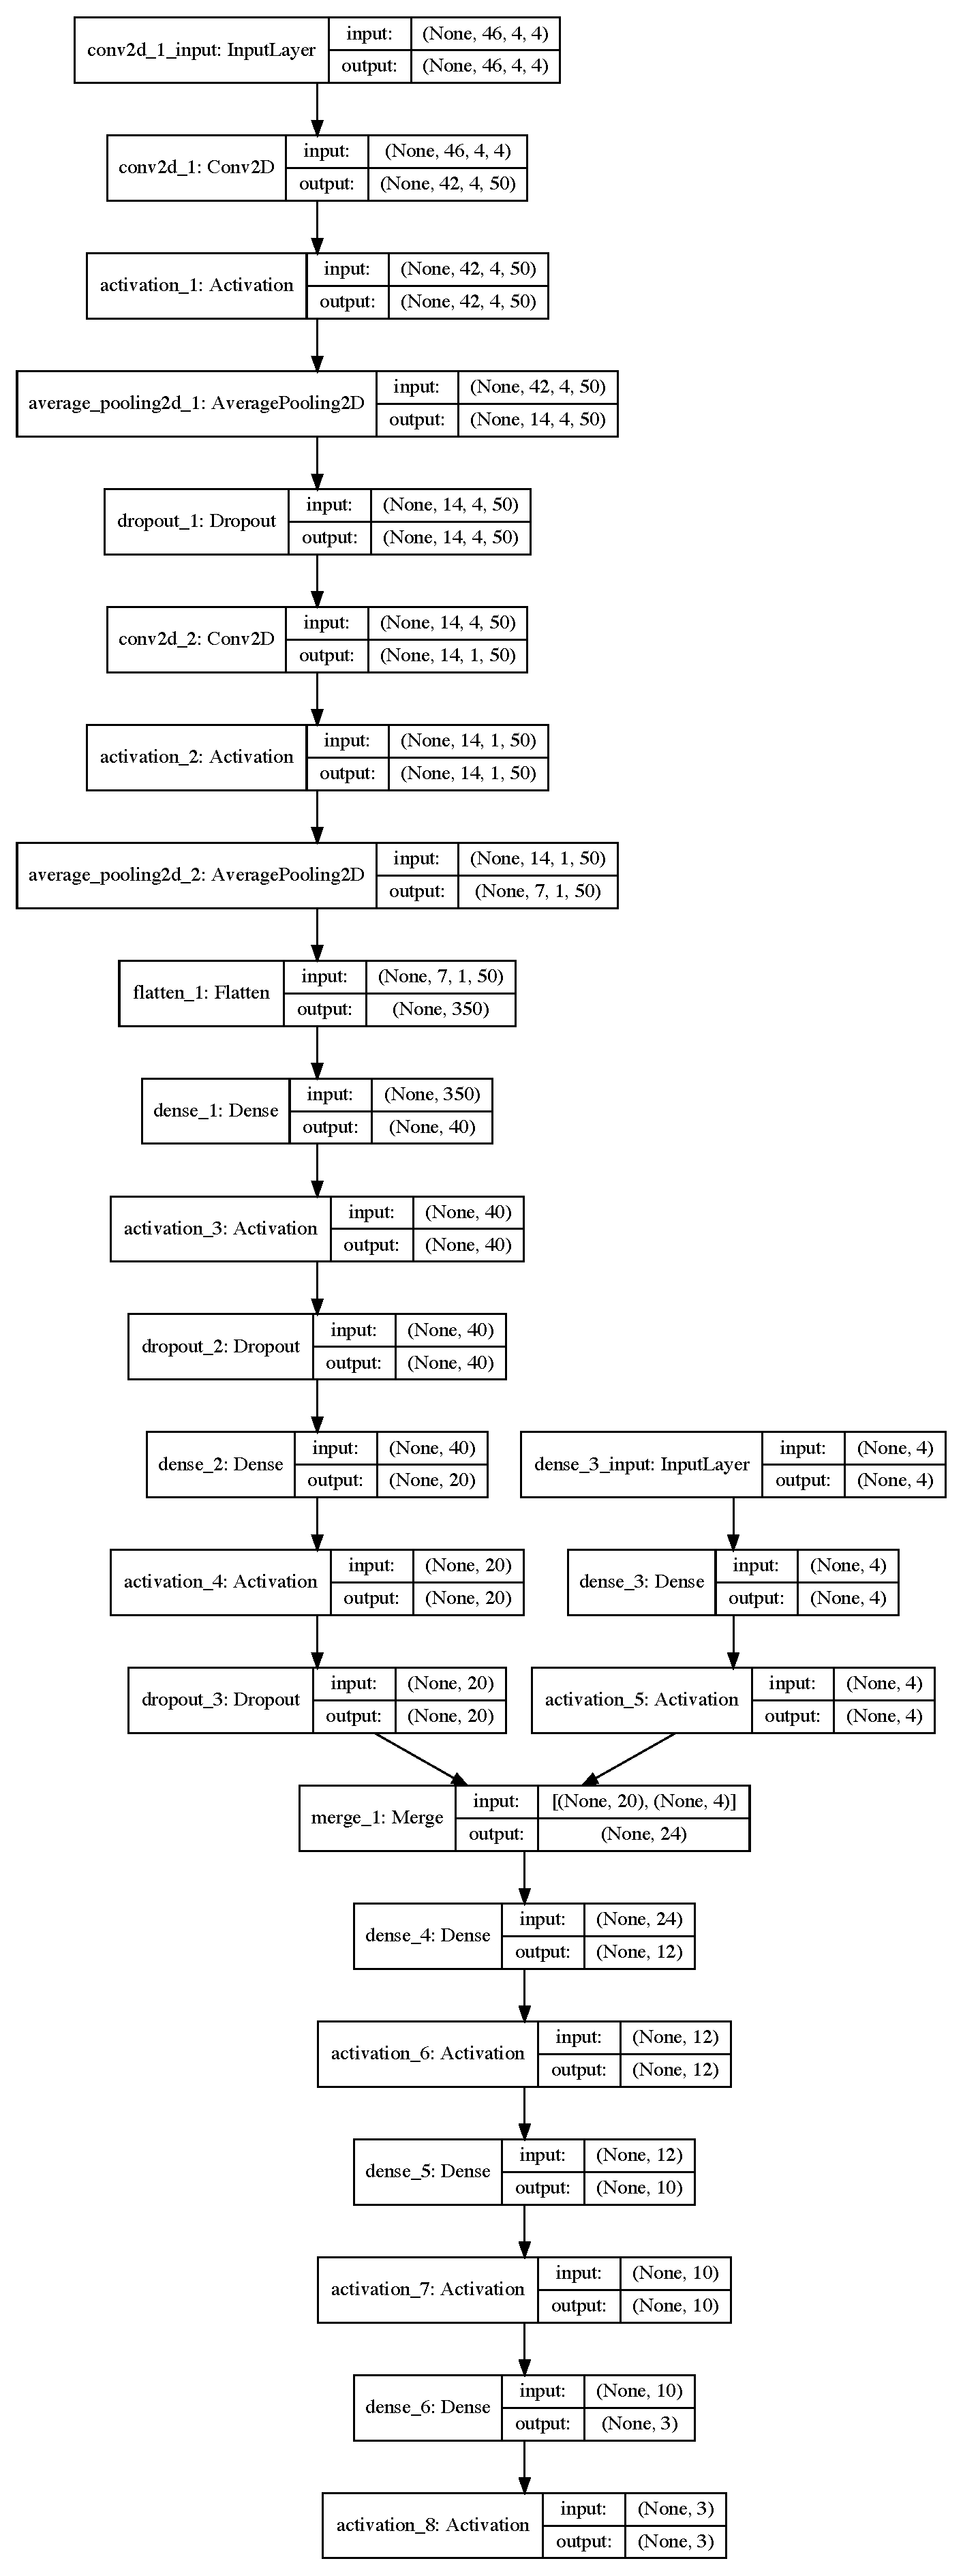
\includegraphics[width=0.6\textwidth]{Figures/Chapter5/SNAGNNoise}
  \caption{The CNN used for classification of SN vs AGN vs Noise. Each layer is labeled with its function within the network as well as its input and output dimentions.}
  \label{fig:AGNNoiseSNModel}
\end{figure}

\subsubsection{Training the model}
The combined training sample build in \sref{sec:AGNNoiseSNSample} is passed through the network using a batch size of 5000 objects with 100 epoch, or individual runs of the backpropagation algorithm. CNNs are often trained on smaller batches of data to accelerate the learning process and help to prevent overfitting. As a general rule of thumb for the choice of the number of the fitting epoch, the fitting is stopped when the model approaches convergence as an excessive number of epochs would allow the model to `learn' the test sample leading to overfitting.

My best model, as described in \sref{sec:AGNNoiseModel}, converges rapidly to the accuracy of 99.7\% which vastly exceeded our expectations. \fref{fig:AGNNoiseROC} shows the Receiver Operating Characteristic (ROC) which is the most commonly used metric of the accuracy of the classification model. The Area Under Curve (AUC) for the ROC has used an indicator that for each individual object's the probability of being a true positive vs a true negative. For this model, I have measured it to be 99.97\%.

\begin{figure}
  \includegraphics[width=\textwidth]{Figures/Chapter5/SNAGNNoiseROC.pdf}
  \caption{ROC curve and the AUC showing the accuracy, reflecting the high quality of the SN vs AGN vs Noise ML model introduce in this section.}
  \label{fig:AGNNoiseROC}
\end{figure}

\subsubsection{Selecting SNe}
After the numerous preparation steps, we can now obtain classifications for each real, unlabelled DES transient. 19,500 objects were sanitised and reshaped using the same method as the training sample before being passed through the classification network. Amongst this sample, 6000 objects received a classification of `most-likely' being a SN, e.g their probability was highest for this label.

To test the classification model and determine a probability threshold that would ensure a high purity of the sample, I use the samples of spectroscopically classified SNIa, CCSN, SLSNe and AGN as a ground-truth sample. Regardless of their subclass, all confirmed SN in the sample were correctly classified using our CNN and all AGN were also correctly accounted for. Furthermore, each confirmed SN has been identified with a very high degree of confidence exceeding 99\% in the worst cases with an average exceeding 99.99\% for the majority of transients. This result confirms that the high degree of accuracy could not be attributed to overfitting or errors in the analysis but was, in fact, the true representation of the quality and the staggering ability for the CNNs to differentiate these classes of transients. The high level of accuracy suggests that a similar project performed on data with lower quality or more incomplete light curves could still result in a positive result paving way for similar methods to be applied in the future astronomical surveys including LSST.

Using the classification probability values measured for the confirmed objects, I set a conservative threshold of 98\% to select objects which are to enter the next stage of my analysis. This retained 5273 objects which are an approximate match to the numbers of SN discoveries expected in DES \citep{Bernstein2012}.

\subsection{Classifying SNe}
Upon the classification of 5273 transients found in the first four years of operation of DES, the next step of the analysis is to attempt to divide these objects into their respective subclasses using only their light curve data. This task is perhaps one of the greatest challenges facing SN surveys to date, with no project ever accomplishing this with a high degree of confidence without the use of reshifting as a modelling prior.

The classification of SN in the absence of the distance prior requires us to focus purely on the morphology of the light curve including its colour and temporal evolution and apparent luminosity as the only available sources of information. These differences may be very subtle for a number of SN classes, most predominantly SN\,Ia and SN\,Ibc, and we, therefore, do not expect to be able to produce a classification model matching the accuracy of that used to identify SN candidates in DES.

\subsubsection{Data preparation and network selection} \label{sec:SNClassificationNetwork}
The training sample used in the classification of SNe is similar to that used in the previous section, albeit consisting of SN light curve only. In order to provide a fair representation for each subclass of objects, I use an equal sample of SN\,Ia, CCSN and SLSN wherein each case 45,000 objects from the training set. In the case of CCSNe, I use an even contribution from both the sample of SN\,II and SN\,Ibc. The data is also sanitised and reshaped using the tools as used in \sref{sec:AGNNoiseSNSample}

To build the SN classification model, I use the approach developed in \sref{sec:AGNNoiseModel} as the benchmark, and modifying that network to suit this more complex problem. Perhaps the most important change was the introduction of the absolute magnitude as one of the input parameters. In the selection of SNe, performed in \sref{sec:AGNNoiseModel}, this was not necessary as the light curve evolution, normalised to one for each object, provides sufficient information to distinguish between these very distinct classes of objects. In the case of SNe, the difference is very subtle relative to the previous model with the luminosity as a function of the colour likely being one of the strongest indicators for each subclass. The absolute luminosity is measured as the maximum flux in each band across all seasons of data. This provides only four additional data point and is, therefore, introduces late into the network in order to provide them with more weight in determining the final classification \fref{fig:SNClassificationNetwork}.

\begin{figure}
  \centering
  \includegraphics[width=0.6\textwidth]{Figures/Chapter5/SN}
  \caption{The CNN used to subclassify DES SNe amongst their spectral subtypes. This network relies on `Tanh' activation funtions and makes use of the information about the apparent luminosity of the SN, differing from that used in \sref{sec:AGNNoiseModel}}
  \label{fig:SNClassificationNetwork}
\end{figure}

Another important change introduces in this iteration of the CNN was an increase in the number of convolutional filters responsible for measuring the colour of the SN. Through a number of iterations of the model, I found that an increase from 30 to 50 unique filters improves the classification rate by $\sim$3\% without overfitting the model.

Finally, one of the biggest improvements in the model came from modifying the activation function to follow the Tanh distribution over ReLU, introducing an improvement of $\sim$5\%. Interestingly, the same behaviour was not previously observed in the SN identification network where the use of Tanh or Sigmoidal activation functions hinders the classification rate. One possible explanation of this comes from the fact that the differences between the objects in the training samples in the SN identification sample are so large that they require a more flexible and forgiving activation function such as ReLU, while the similarity of the SN subclasses requires a very sensitive, high gradient function to be used. The benefit of the Tanh over a Sigmoid is the scaling between the negative and positive unity as opposed to zero and one, which allows for objects with small negative values.

\subsubsection{Training the model} \label{sec:SNClassification}
Using the training sample and the CNN developed in \sref{sec:SNClassificationModel}, I built a SN classification model that, with an accuracy of 90\%, is one of the most successful SN classifiers to date, despite its independence from any distance priors. At the stage of classifying a purified sample of SNe, our result can be directly compared with \citet{Lochner2016}. Our AUC measured at 97.9\% for SN\,Ia marginally exceeds that of the best result found in \citet{Lochner2016}. However, this does not tell the full story as the best model found in their work sufferers largely from overfitting and the more correct value, found using a larger (albeit non-representative of all subclasses) sample is closer to $\sim$85\%. The accuracy of our classifier is again a testament to the power of CNNs, demonstrating that a similar model could be used in future surveys such as LSST.

\begin{figure}
  \includegraphics[width=\textwidth]{Figures/Chapter5/SNROC.pdf}
  \caption{The ROC and AUC measured for the SN photometric classification model shown separately for each class of SN present in our training sample.}
  \label{sec:SNClassificationROC}
\end{figure}

\subsection{SLSNe in DES}
Before the SN classification model can be applied to the sample of DES SN candidates, identified in \sref{sec:SNClassification}, it must first be tested against the ground-truth sample of spectroscopically confirmed objects detected by DES. While the model shows that a high degree of precision, it is possible that mistakes in the creation of the artificial training sample could lead to some subclasses not being represented correctly in the classification model.

\subsubsection{Ground-truth sample} \label{sec:SNTruth}
Amongst the sample of 250 spectroscopically confirmed SN\,Ia, 243 are correctly classified in this work. This, in fact, exceeds the value expected from the raw accuracy figures which are likely explained by the spectroscopically confirmed objects being easier to classify than some objects that may lay at the detection limit of the survey.

With this positive result, I apply the same method to SN\,Ib/c and SN\,II. Here the results begin to shed a light on a major issue uncovered in this section. While a majority of the SN\,Ib/c have been correctly identified, a number of SN\,II is have been misidentified as SLSN. The visual inspection of these objects shows that they are exclusively SN\,IIP with, particularly slow descent times. This is a subclass of objects which was not represented at all in the training sample due to the lack of sufficient data. At the current time, using the data available in the literature is not possible to expand our training set with examples of SN\,IIP. However, in \cref{Chapter6} I investigate other approaches, centred around the concept of Unsupervised ML to separate these two groups of transients and provide a pure sample of SLSN.

As the final check, I test the sample of DES SLSNe and find that only 12 of the 18 objects are fully recovered by the model. While at the first glance, this result appears to be in contradiction with the predicted accuracy of the classifier, two of these objects are knows to be only tentatively classified as SLSN (DES15C3hav, DES14C1rhg). Three objects are known not to be a good match to the magnetar model under any assumptions tested in \sref{sec:MagnetarModel} (DES13S2cmm, DES14S2qri). It is harder to postulate why DES16C3ggu and DES15X1noe are not part of the sample. While is possible that their late-season detection is at fault, however, we see that behaviour from a number of objects which are correctly classified.

\begin{table}
  \caption{Percentage probability of the spectroscopically confirmed DES SLSNe as found in the ML photometric classification presented in this chapter.}
  \label{tab:SLSNTruth}
  \centering
  \begin{tabular}{l|r|r|r}
    SN Name & SN\,Ia & CCSN & SLSN \\
    \hline
    DES13S2cmm & 0.04\,\% & 89.18\,\% & 10.77\,\% \\
    DES15X3hm  & 5.65\,\% & 7.40\,\% & 86.95\,\% \\
    DES14X3taz & 1.71\,\% & 2.25\,\% & 96.04\,\% \\
    DES15S2nr  & 0.01\,\% & 0.54\,\% & 99.46\,\% \\
    DES14C1fi  & 0.00\,\% & 0.11\,\% & 99.89\,\% \\
    DES14X2byo & 0.01\,\% & 0.10\,\% & 99.89\,\% \\
    DES15C3hav & 46.10\,\% & 10.38\,\% & 43.52\,\% \\
    DES14C1rhg & 0.87\,\% & 96.90\,\% & 2.23\,\% \\
    DES14S2qri & 2.92\,\% & 90.66\,\% & 6.43\,\% \\
    DES14E2slp & 0.28\,\% & 1.85\,\% & 97.87\,\% \\
    DES15E2mlf & 0.00\,\% & 0.23\,\% & 99.77\,\% \\
    DES15X1noe & 3.63\,\% & 52.81\,\% & 43.56\,\% \\
    DES15S1nog & 19.93\,\% & 14.05\,\% & 66.02\,\% \\
    DES16C3cv  & 0.00\,\% & 0.04\,\% & 99.96\,\% \\
    DES16C2nm  & 0.00\,\% & 0.05\,\% & 99.95\,\% \\
    DES16C2aix & 0.05\,\% & 46.19\,\% & 53.76\,\% \\
    DES16C3dmp & 9.60\,\% & 3.51\,\% & 86.89\,\% \\
    DES16C3ggu & 85.20\,\% & 11.52\,\% & 3.28\,\%
  \end{tabular}
\end{table}

\subsubsection{SN classification}
I applied the final classification model to the 5273 objects real DES objects, previously identified as SN candidates. At the 50\% accuracy threshold, 3192 objects were identified as SN\,Ia which matches the expected values found in \citep{Bernstein2012}, 1389 objects were identified as CCSN which again does not exceed our expectations. The remaining 509 objects were identified as SLSN.

This largely exceeds the numbers expected from the rate of SLSN and is known to be contaminated with long duration SN\,II. However, as the classification model was shown in \sref{sec:SNTruth} to be able to identify a number of known SLSN with a high degree of accuracy (\tref{SLSNTruth}), we have a strong degree of belief that there are in fact numerous SLSN hidden in this contaminated sample that may be recoverable using further analysis, as presented in \cref{Chapter6}

\section{Summary}
In this chapter, I described the approach used in building a training sample of transients resembling the sample of real transients observed by the DES. I used the SNANA generated sample of SN\,Ia. The CoCo and SLAP packages, developed in \cref{Chapter3}, were used to create samples of CCSN and SLSNe respectively. Furthermore, I use a sample of AGNs generated for a similar study in \citet{Hoenig2014} and a basic model of spurious noise detections to generate a DES-like sample of real transients and their contaminants. I use the approach similar to that found in SNANA to apply the survey noise to the modelled light curves before augmenting them to a uniform cadence using GPR, previously discussed in \sref{sec:Augmentation}.

This training sample was used to develop a classification pipeline for photometrically identifying a sample of real SN candidates in DES. This was performed in conjunction with the state of the art CNN algorithm. A similar approach was subsequently used to create a SN photometric classification tool. Our testing suggests that it is one of the most powerful tools of its kind currently available. I applied it to the DES dataset identifying 3192 SN\,Ia, 1389 potential CCSN and a sample of 500 SLSN, although we understand that this sample is heavily contaminated by SN\,IIP which were not included in the original training sample.
 % Machine Learning

\chapter{Sample of DES SLSNe}
\label{Chapter6}
\lhead{Chapter 6. \emph{High redshift SLSN}}

The aim of this chapter, cultumating the overall goal of this thesis, is the study of a sample of SLSNe in DES. In the previous chapters I identified SLSNe using the magnetar model approach, built an artifial sample of SLSNe, as well as numerous other classes of transients, and constructed a photometric classification of DES SN candidates. This process has identified a large sample of 500 potential SLSN candidates that, while I believe hides a large number of true SLSNe, is heavily contaminated with slowly evolving SN\,IIP.

Here, I begin by examining this dataset in order to separate the events we are interested in through a combination of visual inspection, magnetar model fitting, unsupervised ML as well as the use of the available distance measurements. Through this process I produce a `gold' sample of DES SLSN that contains XX objects with a strong degree of confidence in their classification thanks to the presence of either spectroscopic redshift. Further to this, I produce a `silver' sample containing objects with only [WRITE TYPE] classifications and `bronze' sample which is more speculative but worth exploring in the furthcoming sections.

\section{Purifying the sample of SLSNe}
text

\section{Observational Properties}
text

\section{The Rate of SLSN in DES}
 % Conclusion

%% ----------------------------------------------------------------
% Now begin the Appendices, including them as separate files

\addtocontents{toc}{\vspace{2em}} % Add a gap in the Contents, for aesthetics

\appendix % Cue to tell LaTeX that the following 'chapters' are Appendices

\chapter{Light Curves of SLSNe in DES}
\label{AppendixA}
\lhead{Appendix A. \emph{DES SLSN Light Curves}}

\begin{figure}[H]
  \centering
  \includegraphics[width=\textwidth]{Figures/xkcd/appendix.png}
  \caption*{xkcd.com/552}
\end{figure}

\section{Spectroscopically Confirmed}
Below, I include the light curves of the SLSNe spectroscopic confirmed by DES.

\section{Photometrically Classified}
Below, I include the light curves of SLSNe classified using the ML photometric classification method developed in Chapter \ref{Chapter5}.
	% Appendix Title

\addtocontents{toc}{\vspace{2em}}  % Add a gap in the Contents, for aesthetics
\backmatter

%% ----------------------------------------------------------------
\label{Bibliography}
\lhead{\emph{Bibliography}}  % Change the left side page header to "Bibliography"

% \bibliographystyle{unsrtnat}  % Use the "unsrtnat" BibTeX style for formatting the Bibliography
\bibliographystyle{aasjournal}

% \bibliography{Bibliography}
% \bibliography{Mendeley}
\bibliography{Thesis}
% \bibliographystyle{aasjournal}

% The references (bibliography) information are stored in the file named "Bibliography.bib"

\end{document}  % The End
%% ----------------------------------------------------------------
